\documentclass[a4paper,11pt]{article}
\usepackage[utf8]{inputenc}


%math  
\usepackage{amsmath}
\usepackage{amssymb}
\usepackage{amsfonts}
\usepackage{theorem}
\usepackage{pstricks}
\usepackage{algorithm}
\usepackage{algpseudocode}
\usepackage{enumitem}
\usepackage{ifthen}     % if-then-else command
\usepackage{euscript}
\usepackage{mathrsfs}   % 
\usepackage{tabu}
\usepackage{rotating}
\newtheorem{theorem}{Theorem}[section]     %
\newtheorem{definition}{Definition}[section]  %
\newtheorem{proof}{Proof}[section]  %
\newtheorem{lemma}{Lemma}[section]  %
\newtheorem{proposition}{Proposition}[section] %
\newtheorem{remark}{Remark}[section] %
\DeclareMathOperator{\sgn}{sgn} % enable partial derivative
\usepackage[super]{nth} % enable easy first and second etc
\usepackage{comment} % to enable block of comment
\DeclareMathOperator*{\argmax}{arg\,max} %enable argmax
\DeclareMathOperator*{\argmin}{arg\,min} %enable argmin
\newcommand{\innerproduct}[2]{\langle #1, #2 \rangle} %enable innerproduct

\usepackage{longtable}
\usepackage{pdfpages}

%formatting
\usepackage{hyphenat}
\usepackage{enumerate}  % tm make it possible to define the numbers (A,a, ...)
\usepackage{float}      % you can define 'H' so that floats are forced to be putted 'here'
\usepackage{afterpage}  % adds \afterpage command, which makes it possible to issue \afterpage{\clearpage} which flushes all floats after this page
\usepackage{rotating}
\usepackage{ulem}       % for underlining text \ul{...}
\usepackage{derivative} % for partial deivative

%graphics
\usepackage{epic,eepic}
\usepackage{graphicx}
\usepackage{epstopdf}
\usepackage{caption}
\usepackage{subcaption}
\usepackage{tabularx}
\usepackage{bigstrut}
\usepackage{color, xcolor}

% code
\usepackage[framed,numbered,autolinebreaks,useliterate]{mcode}

%tables
\usepackage{listings}
\usepackage{tabularx}
\usepackage{multirow}   % multirow{nrows}[bigstruts]{width}[fixup]{text} multirow cells
\usepackage{listings}
\usepackage{hhline}     % generates nicer table lines (without missing pixels) + more flexible
\usepackage{colortbl}   % for coloured columns
\usepackage{threeparttable} % adds the possibility to add footnotes in tables
\usepackage{longtable}  %for tables spanning multiple pages

%referencing
\usepackage{cite}
\usepackage{bbm}
\usepackage{url}
\usepackage{hyperref}
\hypersetup{colorlinks=true,
            citecolor=black,
            linkcolor=red,
            citebordercolor=blue,
            urlcolor=magenta,
            linktocpage,
            plainpages=false}
\usepackage{listings}
\usepackage{comment}
\numberwithin{equation}{section} % for the formulas order

%Matlab code
\usepackage{listings}
%\usepackage[framed,numbered,autolinebreaks,useliterate]{mcode}

%----------------------
\PassOptionsToPackage{normalem}{ulem}
\topmargin 0.4cm
\oddsidemargin -0.1cm
\textwidth  15cm
\headheight 0.0cm
\textheight 22.2cm
\parindent  0mm
\parskip    10pt
\tolerance  1000
%----------------------

\title{Technical Report}
\author{Theodors Katzalis}
\date{March 2023}

\begin{document}

\maketitle

\tableofcontents
\newpage

\section{Introduction}
\label{intro}

\subsection{Study Phase} (this subsection can be remove in final report)

Part 1: Line Search methods

\begin{itemize}
\item Chapter 1 and Chapter 2 of ref.1
\item Chapter 3 : Sections 3.1, 3.2, 3.3 and 3.5 of ref.1
\item Zhang, H. and Hager, W.W. (2004) A Nonmonotone Line Search Technique and Its Application to Unconstrained Optimization. SIAM Journal on Optimization, 14, 1043-
1056.
\end{itemize}

Part 2: Quasi-Newton methods
\begin{itemize}
\item Chapter 6 : Sections 6.1 and 6.4 of ref.1
\item Chapter 7 : Section 7.2 of ref.1
\item Chapter 2 : Section 2.2 of ref.2
\end{itemize}

Part 3: L-BFGS-B
\begin{itemize}

\item Byrd, R. H.; Lu, P.; Nocedal, J.; Zhu, C. (1995). A Limited Memory Algorithm for
Bound Constrained Optimization. SIAM J. Sci. Comput. 16 (5): 1190–1208.
doi:10.1137/0916069. S2CID 6398414.

\item Zhu, C.; Byrd, Richard H.; Lu, Peihuang; Nocedal, Jorge (1997). L-BFGS-B: Algorithm 778: L-BFGS-B, FORTRAN routines for large scale bound constrained optimization. ACM Transactions on Mathematical Software. 23 (4): 550–560.

\item Morales, J. L.; Nocedal, J. (2011). Remark on quote;algorithm 778: L-BFGS-B: 
Fortran subroutines for large-scale bound constrained optimization; ACM Transactions on Mathematical Software. 38: 1–4.

\end{itemize}

References
\begin{itemize}
 \item Ref. 1: Numerical optimization, J. Nocedal and S. Wright, Second Edition (digital copy of the book can be found \url{https://www.csie.ntu.edu.tw/~r97002/temp/num_optimization.pdf}
\item Ref. 2: Nonlinear programming, D. Bertsekas, Third Edition, Athena Scientfic.
\end{itemize}

Knowledge consolidation of math optimization around Quasi-Newton methods via concept summarizing and exercises solving of \cite{nocedal1999numerical, bertsekas1997nonlinear}.

\subsection{Updates}
\begin{itemize}
    \item \textbf{Week 11-18/04/2023:} 
    \begin{itemize}
        \item Add documentation to the functions `newton.m` and `steepest\_descent.m` with examples on how to use it. Otherwise, the jupyter notebook can be used as a reference point on how to call these methods.
        \item Add wolfe strong line search method. For the interpolation step, we use the simple bisection method instead of a more sophisticated solution with cubic or quadratic interpolation.
        \item Add more functions with more than 2 dimensions as provided on mattermost to test the functions.
        \item Add plots when finishing the executing of the line search methods to illustrate the progress of the algorithm.
        \item The jupyter notebook has been updated to include the new functions and to show the plots. (Currently a pdf is exported to include it on this report. When there is access to a git host system, a link will be used to avoid the sync issue).
    \end{itemize}
    \item \textbf{Week 18-27/04/2023:}
    \begin{itemize}
        \item Document how to execute the functions and provide a demo script along with the jupyter notebook (moved to appendix).
        \item Use new starting points.
        \item Draw 3d plots using contour and 3d lines.
        \item Create a table with the results of the analysis.
    \end{itemize}
    \item \textbf{Week 28-04/05/2023:}
    \begin{itemize}
        \item Implement the nonmonotone line search technique of Zhang-Hager.
    \end{itemize}
    \item \textbf{Week 05-11/05/2023:}
    \begin{itemize}
        \item Implement the nonmonotone line search technique of Grippo.
        \item Implement the bisection wolfe weak condition and replace it with the faulty backtracking wolfe weak implementation.
        \item Add Goldstein condition as a curvature condition. Mimic the wolfe weak implementation.
        \item Automate simulation of all the possible combinations of line search techniques and step sizes and create a csv file
        \item Create tables for the results of the above simulation, converting csv to tex tables.
        \item Improve performance of simulations, by using the \verb|function_handle| to convert symbolic functions to function handlers.
    \end{itemize}
    \item \textbf{Week 11-15/05/2023:}
    \begin{itemize}
        \item Document inexact line/step length search strategies (wolfe, armijo, goldstein) and type of conditions (sufficient, curvature)
        \item Add number of function evaluations and number of gradient of function evaluations as metrics for the simulations
    \end{itemize}
    \item \textbf{Week 15-25/05/2023:}
    \begin{itemize}
        \item Debugging divergence of algorithms (+ why are we getting imaginary numbers?).
        \item Adjust the initial alpha value to be within boundaries so the value $x+a*pk$ stays within function's domain.
        \item Add more conclusions about the behaviour of the optimization algorithms.
    \end{itemize}
\end{itemize}
 
\pagebreak

\section{Theoretical Experiments}

Problems listed on Chapter 2 of ref \cite{nocedal1999numerical}:

\label{rosenbrock}
\subsection{}

\textbf{Problem}

Compute the gradient $\nabla f(x)$ and Hessian $\nabla^2 f(x)$ of the Rosenbrock function.

\begin{equation}
    f(x) = 100(x_2 -x_1^2)^2 + (1-x_1)^2 
\end{equation}

Show that $x^{\ast} = (1, 1)^{T}$ is the only local minimizer of this function, and that the Hessian matrix at that point is positive definite.


\textbf{Solution}

\begin{align}
    \nabla f(x) &= (\frac{\partial f}{\partial x_1}, \frac{\partial f}{\partial x_2}) \\
    \nabla f(x) &= (2(200x_1^3 -200x_2x_1 + x_1- 1)), 200(x_2 - x_1^2)) \\
    \nabla^2 f(x) &= 
    \begin{bmatrix}
    800x_1^2 - 400(x_2 - x_1^2) +2 & -400x_1 \\
    -400x_1 & 200
    \end{bmatrix}
\end{align}

To find all the possible stationary points and potentially the local minimums we solve $\nabla f(x) =0$ and the only root is $x^{*} = (1,1)$. To check if the stationary point is a local minimum and this case a global minimum, since there aren't any other stationary points, then we have to check if $\nabla^2 f(x^{*})$ is positive definitive and we have:

\begin{equation}
    \nabla^2 f(1,1) = 
    \begin{bmatrix}
        802 & -400 \\
        -400 & 200
    \end{bmatrix}
\end{equation}

The eigenvalues for the above matrix are $\lambda_1 \approx 1001.6$ and $\lambda_2 \approx 0.399361$. We can prove that the matrix is positive definite. Thus, the $x^{*} = (1,1)$ is the global minimum of the Rosenbrock function.

\subsection{}

\textbf{Problem}

Show that the function $f(x) = 8x_1 + 12x_2 + x_1^2 - 2x_2^2$ has only one stationary
point, and that it is neither a maximum or minimum, but a saddle point. Sketch the contour
lines of f.

\textbf{Solution}


To find the stationary points we solve $\nabla f(x) = 0$ and we have:
\begin{equation}
    \nabla f(x) = (2(x+4), -4(y-3)
\end{equation}
, thus the only root is $x^{*} = (-4, 3)$. To prove that it is a saddle point, we have to show that some of the eigenvalues of the Hessian matrix are positive and the rest negative. Thus we have:

\begin{equation}
    \nabla^2 f(x) = 
    \begin{bmatrix}
        2 & 0 \\
        0 & -4
    \end{bmatrix}
\end{equation}

and eigenvalues $\lambda_1 = -4$ and $\lambda_2 = 2$. The first is positive and the second is negative. Thus, we have proved that the point $(-4, 3)$ is a saddle one.

\begin{figure}[h!]
     \centering
     \begin{subfigure}[b]{0.45\textwidth}
         \centering
         \includegraphics[width=\textwidth]{assets/saddle_3d.png}
         \caption{3D}
     \end{subfigure}
     \hfill
     \begin{subfigure}[b]{0.45\textwidth}
         \centering
         \includegraphics[width=\textwidth]{assets/saddle_contour.png}
         \caption{Contour lines}
     \end{subfigure}
    \caption{}
\end{figure}

\subsection{}

\textbf{Problem}

Let a be a given n-vector, and A be a given n × n symmetric matrix. Compute the
gradient and Hessian of $f_1(x) = a^T x$ and $f_2(x) = x^TAx$.

\textbf{Solution}

For the $f_1$, we have:

\begin{align}
    \nabla f_1(x) &= a \\
    \nabla^2 f_1(x) &= 0
\end{align}

, due to the fact that the vector $a$ is constant.

For the $f_2$, we have:

\begin{align}
    \nabla f_2(x) &= 2Ax \\
    \nabla^2 f_2(x) &= 2A
\end{align}

\subsection{}

\textbf{Problem}

Write the second-order Taylor expansion (2.6) for the function cos(1/x) around
a nonzero point x, and the third-order Taylor expansion of cos(x) around any point x. Evaluate the second expansion for the specific case of x = 1.

\textbf{Solution}

For the second order taylor expansion of $cos(1/x)$ near the point $x_0$ we have:

\begin{equation}
cos(1/x)) = cos(1/x_0) + \frac{sin(1/x_0)}{x_0^2 (x-x_0)} - \frac{1}{2} \frac{2x_0*sin(1/x_0) + cos(1/x_0)}{x_0^4(x-x_0)^2}
\end{equation}

For the third order taylor expansion of $cos(x)$ near the point $x_0$, we have:

\begin{equation}
    cos(x) = cos(x_0) - (x-x_0)sin(x_0) - \frac{(x-x_0)^2}{2}cos(x_0) + \frac{(x-x_0)^3}{6}sin(x_0)
\end{equation}

\subsection{}

\textbf{Problem}

Consider the function f: $R^2 \rightarrow R$ defined by $f(x) = {||x||}^2$. Show that the sequence of iterates {$x_k$} defined by

\[x_k = (1 + \frac{1}{2^k}) \begin{bmatrix}
    cosk \\ sink
\end{bmatrix}\]

satisfies $f(x_{k+1} < f(x_k)$ for k = 0, 1, 2, .... Show that every point on the unit circle $\{x | {||x||}^2 = 1\}$ is a limit point for {$x_k$}.

\textbf{Solution}

\begin{align}
    f(x_k) &= (1+\frac{1}{2^k})^2(cos^2k + sin^2k) \\
    f(x_k) &= (1+\frac{1}{2^k})^2
\end{align}

For the inequality, we have:

\begin{align}
    f(x_{k+1}) &< f(x_k) \\
    (1 + \frac{1}{2^{k+1}})^2 &< (1 + \frac{1}{2^k})^2 \\ 
    k+1 &> k
\end{align}

, that is true.

Also, because $\lim_{k\to\infty} f(x_k) = 1$ and $f(x_{k+1}) < f(x_k)$, the points of the unit circle are limit points for {$x_k$}.

\subsection{}

\textbf{Problem}

Prove that all isolated local minimizers are strict. (Hint: Take an isolated local
minimizer $x^{*}$ and a neighborhood N . Show that for any $x \in N$ , $x \neq x^{*}$ we must have $f(x) > f(x^{*})$.)

\textbf{Solution}

By definition a point $x^{*}$ of $f$ is strict when there is a neighborhood N such that $f(x^{*}) < f(x)$ for all $x \in N$ with $x \neq x^{*}$.

By definition a point $x^{*}$ is an isolated local minimizer if there is a neighborhood N of $x^{*}$ such that the $x^{*}$ is the only local minimizer in N.

Let's suppose that given an isolated local minimer $x^{*}$ for a neighbor N, then $f(x) \leq f(x^{*})$ for $x \in N$ and $x \neq x^{*}$. Then the minimizer $x^{*}$ isn't the only one, thus isn't isolated. Thus it should be $f(x) > f(x^{*})$. The last one completes the definition of a strict minimizer. Thus we have proved that an isolated minimer is a strict one.




\section{Numerical Experiments}

In this section, we will test well-known optimization techniques with multiple step size strategies on a different set of functions. 
The in-house implementation of the above can be found at the \ref{code}.
For an example on how to use the functions you can check the \verb|demo.m| and the jupyter notebook.

The line search techniques are based on the simple iterative formula of $x_{k+1} = x_k + a_k pk$, where $p_k$ is the direction vector and $a_k$ is the step size. For the $pk$, we will study two main schools of thought, the newton method and the steepest descent. On the other hand for the step size, we will study many different approaches such as (\verb|grippo|, \verb|Hanger and Zhang|, \verb|backtracking|, \verb|bisection wolfe weak|, \verb|wolfe strong|, \verb|goldstein|). 

Our goal is to find $a_k$ that minimizes the function $\phi (a) = f(x_k + a pk)$. To find an exact answer is computationally expensive, so usually inexact search strategies are incorporated. Typical step size search algorithms try out a sequence of candidate values for $\alpha$, stopping to
accept one of these values when certain conditions are satisfied.
An effective condition that leads to a decrease of a function while ensuring convergence, is the so called \textbf{sufficient decrease condition}:

\begin{equation}
f(x_k + a p_k) \leq f(x_k) + a  c_1 p_k^T \nabla f_k
\end{equation}

This condition is also called \textbf{Armijo condition}, where $c_1 \in (0,1)$.

The sufficient decrease condition is not enough by itself to ensure that the algorithm
makes reasonable progress. To rule out unacceptably short steps we introduce a second requirement,
called the \textbf{curvature condition}, which requires $a_k$ to satisfy:

\begin{equation}
c_2 \nabla f_k^Tp_k \le \nabla f(x_k + a p_k)^T p_k
\end{equation}

, where $c2 \in (c_1,1)$. The sufficient decrease and curvature conditions are known collectively as the \textbf{Wolfe
conditions}.

There is also another similar pair of conditions called the \textbf{strong Wolfe} conditions:

\begin{align}
f(x_k + a p_k) &\leq f(x_k) + a  c_1 p_k^T \nabla f_k \\
|\nabla f(x_k + a p_k)^T p_k| &\le c_2  |\nabla f_k^Tp_k|
\end{align}

The only difference with the Wolfe conditions is that we no longer
allow the derivative $\nabla f(x_k + a_k  p_k)$ to be too positive. Hence, we exclude points that are far from stationary points of $f(x_k + a_k p_k)$.


Like the Wolfe conditions, the \textbf{Goldstein} conditions ensure that the step length $\alpha$
achieves sufficient decrease but is not too short. The Goldstein conditions can also be stated
as a pair of inequalities, in the following way:

\begin{align}
    f(x_k + a_k pk) &\leq f(x_k) + a_k c \nabla f_k^T p_k \\
    f(x_k) + a_k (1-c) \nabla f_k^T p_k & \le f(x_k + a_k p_k) 
\end{align}

, where $0 < c < 1/2$. The first inequality is the sufficient decrease, and similarly with the Wolfe, the second one can be assumed as the curvature condition. A key difference between the Wolfe and the Goldstein conditions is that for the first there are two independent variables to configure $c_1$ and $c_2$, but for the second, only one $c$.


% The steps are:
% \begin{itemize}
%     \item Include all the ".m" files in the path (\verb|addpath()|)
%     \item Define a symbolic function
%     \item Pick a number from 1-4 to choose your step size configuration (1: Backtracking wolfe weak, 2: Wolfe stong, 3: Backtracking armijo, 4: None)
%     \item Pick a starting point e.g. \verb|[1,1]'|
%     \item Pick a search domain for the plots e.g. \verb|search_x = -1:-0.1:1|, \verb|search_y = -1:0.1:1|
% \end{itemize}

\subsection{}


Test on problem functions 1: Ext; Rosenbrock, 2: Wood, 3: Powell singular, 4: Cube, 5: Trigonometric, 6: Helical valley (ref. page 713 Grippo), the following line search techniques:
    
\begin{itemize}
    \item Grippo/max with Armijo
    \item Grippo/max with Armijo + Goldstein (lower bound)
    \item Grippo/max with Wolfe condition (open)
    \item Comparison with Hagher \& Zhang with Steepest descent \& Newton: a) Armijo, b) Wolfe
    \item Comparison with monotone Armijo + Goldstein
\end{itemize}

\begin{align*}
    rosen(n) &= \sum_{i=1}^{n-1} [100 (x_{i+1}-x_i^2)^2 + (1-x_i)^2], \\ &\quad x_0 = [-1.2,1,...,-1.2,1], \quad f_{min}(1,1,...,1,1)=0  \\
    wood(x_1,x_2,x_3,x_4) &= 100*(x_1^2-x_2)^2 + (x_1-1)^2 + (x_3-1)^2 + 90*(x_3^2 - x_4)^2 + \\ & 10.1*((x_2-1)^2 + (x_4-1)^2) + 19.8*(x_2-1)*(x_4-1)\\ & \quad x_0 [-3,-1,-3,-1], \quad f_{min}(1,1,1,1) = 0 \\
    powell(x_1,x_2,x_3,x_4) &= (x_1+10*x_2) + 5*(x_3-x_4)^2 + (x_2-2*x_3)^4 + 10*(x_1-x_4)^2 \\ & \quad x_0 = [3,-1.0,1], \quad f_{min}(0,0,0,0) = 0 \\
    cube(x_1,x_2) &= 100(x_2-x_1^3)^2 + (1-x_1)^2 \\ & \quad x_0 = [-1.2,-1], \quad f_{min}(1,1) = -6.4931 \\ 
    trig(n) &= \sum_{i=1}^{n}[n + i(1-cosx_i) - sinx_i - \sum_{j=1}^{n}cosx_j]^2,\\ & \quad x_0 = [1/5n,...1/5n], \quad f_{min}(0,...,0) = 0 \\
    helical(x_1,x_2,x_3) &= 100[(x_3-10\theta)^2 + (\sqrt{x_1^2+x_2^2}-1)^2] + x_3^2, \\ & \quad x_0 = [-1,0,0], \quad f_{min}(1,0,0) = 0 \\
\end{align*}

For the results, check the \ref{simulation2}.

\subsubsection{Numerical Results}
\label{simulation2}

\begin{table}[h!]
\resizebox{1.2\textwidth}{!}{
\begin{tabular}{|l|l|l|l|l|l|l|l|}
        method & step size & iterations & $n_{f\_eval}$ & $n_{fgrad\_eval}$ &error x1 & error x2 & error fvalue \\ \hline
newton & backtracking\_armijo & 22 & 47 & 65 & 4.24660306919122e-13 & 1.12310161171081e-12 & 7.67593985588231e-24 \\
        newton & wolfe\_strong & 51 & 100 & 3 & 3.11202148495227e-08 & 6.36384759333808e-08 & 1.16392137900027e-15 \\
        newton & bisection\_wolfe\_weak & 22 & 70 & 93 & 5.99457150585181e-11 & 1.21124443808185e-10 & 3.74552103013306e-21 \\
        newton & bisection\_goldstein & 22 & 94 & 65 & 4.24660306919122e-13 & 1.12310161171081e-12 & 7.67593985588231e-24 \\
        newton & hanger\_zhang\_backtracking\_armijo & 14 & 31 & 41 & 2.84747523005002e-07 & 5.69499220337555e-07 & 8.10811536683049e-14 \\
        newton & hanger\_zhang\_bisection\_wolfe\_weak & 14 & 44 & 60 & 2.84747523005002e-07 & 5.69499220337555e-07 & 8.10811536683049e-14 \\
        newton & hanger\_zhang\_wolfe\_strong & 51 & 99 & 3 & 3.11202148495227e-08 & 6.36384759333808e-08 & 1.16392137900027e-15 \\
        newton & hanger\_zhang\_bisection\_goldstein & 14 & 63 & 41 & 2.84747523005002e-07 & 5.69499220337555e-07 & 8.10811536683049e-14 \\
        newton & grippo\_backtracking\_armijo & 12 & 26 & 35 & 2.72405598078507e-09 & 5.44812550629103e-09 & 7.42048100479684e-18 \\
        newton & grippo\_bisection\_wolfe\_weak & 12 & 37 & 50 & 2.72405598078507e-09 & 5.44812550629103e-09 & 7.42048100479684e-18 \\
        newton & grippo\_wolfe\_strong & 51 & 99 & 3 & 3.11202148495227e-08 & 6.36384759333808e-08 & 1.16392137900027e-15 \\
        newton & grippo\_bisection\_goldstein & 12 & 52 & 35 & 2.72405598078507e-09 & 5.44812550629103e-09 & 7.42048100479684e-18 \\
        steepest & backtracking\_armijo & 500 & 5461 & 1000 & 0.00405416292135397 & 0.00815184029746874 & 1.65095599806295e-05 \\
        steepest & wolfe\_strong & 500 & 5350 & 1879 & 0.0300579681598293 & 0.0570633835894122 & 0.00136533218669946 \\
        steepest & bisection\_wolfe\_weak & 500 & 5935 & 5935 & 0.0287331493832927 & 0.0566851213380007 & 0.000825791155540352 \\
        steepest & bisection\_goldstein & 500 & 10922 & 1000 & 0.00405416292135397 & 0.00815184029746874 & 1.65095599806295e-05 \\
        steepest & hanger\_zhang\_backtracking\_armijo & 500 & 5675 & 1000 & 0.23472734818543 & 0.470226795218939 & 0.350215634074376 \\
        steepest & hanger\_zhang\_bisection\_wolfe\_weak & 500 & 6310 & 6311 & 0.311104956356103 & 0.750437046172376 & 0.195638933287011 \\
        steepest & hanger\_zhang\_wolfe\_strong & 500 & 5263 & 2000 & 0.314048326197008 & 0.632043823210959 & 0.995041070744439 \\
        steepest & hanger\_zhang\_bisection\_goldstein & 500 & 11351 & 1000 & 0.23472734818543 & 0.470226795218939 & 0.350215634074376 \\
        steepest & grippo\_backtracking\_armijo & 500 & 5264 & 1000 & 0.215306188675822 & 0.833536550271171 & 12.7603891154691 \\
        steepest & grippo\_bisection\_wolfe\_weak & 500 & 6588 & 7039 & 1.75378106151133 & 6.75103803591349 & 5.88901289497424 \\
        steepest & grippo\_wolfe\_strong & 500 & 5407 & 1600 & 1.52775558238082 & 4.13459755973619 & 159.824169217124 \\
        steepest & grippo\_bisection\_goldstein & 500 & 10979 & 1000 & 0.215306188675822 & 0.833536550271171 & 12.7603891154691 \\
\end{tabular}}
\caption{rosen(2)}
\label{table:rosen(2)}
\end{table}

\begin{table}[h!]
\resizebox{1.2\textwidth}{!}{
\begin{tabular}{|l|l|l|l|l|l|l|l|}
        method & step size & iterations & $n_{f\_eval}$ & $n_{fgrad\_eval}$ &error x1 & error x2 & error fvalue \\ \hline
newton & backtracking\_armijo & 33 & 70 & 98 & 1.22124532708767e-15 & 7.45181694128405e-13 & 4.84829425702435e-25 \\
        newton & wolfe\_strong & 57 & 112 & 3 & 1.99326337265873 & 0.0116074749287336 & 3.98657911234714 \\
        newton & bisection\_wolfe\_weak & 33 & 102 & 136 & 1.22124532708767e-15 & 7.45181694128405e-13 & 4.84829425702435e-25 \\
        newton & bisection\_goldstein & 33 & 140 & 98 & 1.22124532708767e-15 & 7.45181694128405e-13 & 4.84829425702435e-25 \\
        newton & hanger\_zhang\_backtracking\_armijo & 28 & 53 & 83 & 2.05452321822008e-11 & 1.08046921409866e-08 & 3.87790640761083e-17 \\
        newton & hanger\_zhang\_bisection\_wolfe\_weak & 28 & 80 & 110 & 2.05452321822008e-11 & 1.08046921409866e-08 & 3.87790640761083e-17 \\
        newton & hanger\_zhang\_wolfe\_strong & 57 & 111 & 3 & 1.99326337265873 & 0.0116074749287336 & 3.98657911234714 \\
        newton & hanger\_zhang\_bisection\_goldstein & 28 & 107 & 83 & 2.05452321822008e-11 & 1.08046921409866e-08 & 3.87790640761083e-17 \\
        newton & grippo\_backtracking\_armijo & 28 & 54 & 83 & 2.05452321822008e-11 & 1.08046921409866e-08 & 3.87790640761083e-17 \\
        newton & grippo\_bisection\_wolfe\_weak & 28 & 81 & 110 & 2.05452321822008e-11 & 1.08046921409866e-08 & 3.87790640761083e-17 \\
        newton & grippo\_wolfe\_strong & 57 & 105 & 3 & 1.99326337265873 & 0.0116074749287336 & 3.98657911234714 \\
        newton & grippo\_bisection\_goldstein & 28 & 108 & 83 & 2.05452321822008e-11 & 1.08046921409866e-08 & 3.87790640761083e-17 \\
        steepest & backtracking\_armijo & 500 & 5519 & 1000 & 0.00825312313406334 & 0.98637623229373 & 1.46242950495646 \\
        steepest & wolfe\_strong & 500 & 5024 & 2000 & 0.0107731637582776 & 0.996191710149255 & 1.85334611188857 \\
        steepest & bisection\_wolfe\_weak & 500 & 5942 & 5942 & 0.010206772454277 & 0.995955421443621 & 1.84357300181849 \\
        steepest & bisection\_goldstein & 500 & 11038 & 1000 & 0.00825312313406334 & 0.98637623229373 & 1.46242950495646 \\
        steepest & hanger\_zhang\_backtracking\_armijo & 500 & 4404 & 1000 & 0.964746380583421 & 0.998949846215794 & 19.5357016905797 \\
        steepest & hanger\_zhang\_bisection\_wolfe\_weak & 500 & 4953 & 4954 & 0.852002828801638 & 1.00486216579194 & 11.5403739859886 \\
        steepest & hanger\_zhang\_wolfe\_strong & 500 & 3953 & 2000 & 0.852002828801638 & 1.00486216579194 & 11.5403739859886 \\
        steepest & hanger\_zhang\_bisection\_goldstein & 500 & 8809 & 1000 & 0.964746380583421 & 0.998949846215794 & 19.5357016905797 \\
        steepest & grippo\_backtracking\_armijo & 500 & 4765 & 1000 & 0.156694202405539 & 0.817782719578344 & 895.188811514486 \\
        steepest & grippo\_bisection\_wolfe\_weak & 500 & 5265 & 5716 & 0.223056841897629 & 1.9383515998147 & 408.959889680481 \\
        steepest & grippo\_wolfe\_strong & 500 & 4318 & 2000 & 1.30150442734769 & 0.644113748547448 & 187.000442393963 \\
        steepest & grippo\_bisection\_goldstein & 500 & 9981 & 1000 & 0.156694202405539 & 0.817782719578344 & 895.188811514486 \\
\end{tabular}}
\caption{rosen(10)}
\label{table:rosen(10)}
\end{table}

\begin{table}[h!]
\resizebox{1.2\textwidth}{!}{
\begin{tabular}{|l|l|l|l|l|l|l|l|}
        method & step size & iterations & $n_{f\_eval}$ & $n_{fgrad\_eval}$ &error x1 & error x2 & error fvalue \\ \hline
newton & backtracking\_armijo & 37 & 75 & 110 & 1.99328610095272 & 1.27616560010591e-05 & 3.98662385426169 \\
        newton & wolfe\_strong & 73 & 144 & 3 & 1.99328610095485 & 1.27605656692342e-05 & 3.9866238542612 \\
        newton & bisection\_wolfe\_weak & 38 & 114 & 153 & 1.99328610095495 & 1.2760514065735e-05 & 3.9866238542612 \\
        newton & bisection\_goldstein & 37 & 150 & 110 & 1.99328610095272 & 1.27616560010591e-05 & 3.98662385426169 \\
        newton & hanger\_zhang\_backtracking\_armijo & 34 & 65 & 101 & 1.99328610095495 & 1.27605144084608e-05 & 3.9866238542612 \\
        newton & hanger\_zhang\_bisection\_wolfe\_weak & 34 & 98 & 134 & 1.99328610095495 & 1.27605144084608e-05 & 3.9866238542612 \\
        newton & hanger\_zhang\_wolfe\_strong & 73 & 143 & 3 & 1.99328610095485 & 1.27605656692342e-05 & 3.9866238542612 \\
        newton & hanger\_zhang\_bisection\_goldstein & 34 & 131 & 101 & 1.99328610095495 & 1.27605144084608e-05 & 3.9866238542612 \\
        newton & grippo\_backtracking\_armijo & 34 & 66 & 101 & 1.99328610095495 & 1.27605144084608e-05 & 3.9866238542612 \\
        newton & grippo\_bisection\_wolfe\_weak & 34 & 99 & 134 & 1.99328610095495 & 1.27605144084608e-05 & 3.9866238542612 \\
        newton & grippo\_wolfe\_strong & 73 & 121 & 3 & 1.99328610095485 & 1.27605656692342e-05 & 3.9866238542612 \\
        newton & grippo\_bisection\_goldstein & 34 & 132 & 101 & 1.99328610095495 & 1.27605144084608e-05 & 3.9866238542612 \\
        steepest & backtracking\_armijo & 500 & 5458 & 1000 & 0.00873137703012605 & 0.980465841240178 & 11.4755396870366 \\
        steepest & wolfe\_strong & 500 & 5019 & 2000 & 0.0147750390506268 & 0.989084606184031 & 12.2042583300821 \\
        steepest & bisection\_wolfe\_weak & 500 & 5832 & 5832 & 0.0143203696842829 & 0.988931546483533 & 12.1529570648515 \\
        steepest & bisection\_goldstein & 500 & 10916 & 1000 & 0.00873137703012605 & 0.980465841240178 & 11.4755396870366 \\
        steepest & hanger\_zhang\_backtracking\_armijo & 500 & 4465 & 1000 & 0.912402057567217 & 0.990851320950918 & 31.6212167798638 \\
        steepest & hanger\_zhang\_bisection\_wolfe\_weak & 500 & 5209 & 5210 & 0.912873024059725 & 0.989789465693517 & 103.485831889059 \\
        steepest & hanger\_zhang\_wolfe\_strong & 500 & 4209 & 2000 & 0.912873024059725 & 0.989789465693517 & 103.485831889059 \\
        steepest & hanger\_zhang\_bisection\_goldstein & 500 & 8931 & 1000 & 0.912402057567217 & 0.990851320950918 & 31.6212167798638 \\
        steepest & grippo\_backtracking\_armijo & 500 & 5053 & 1000 & 0.239117413042833 & 0.989791576118572 & 600.936604170597 \\
        steepest & grippo\_bisection\_wolfe\_weak & 500 & 5514 & 5965 & 1.36091792710484 & 0.989791576165746 & 1392.31664495257 \\
        steepest & grippo\_wolfe\_strong & 500 & 4604 & 2000 & 0.0551613732345311 & 0.989791134189679 & 1134.79210579761 \\
        steepest & grippo\_bisection\_goldstein & 500 & 10557 & 1000 & 0.239117413042833 & 0.989791576118572 & 600.936604170597 \\
\end{tabular}}
\caption{rosen(20)}
\label{table:rosen(20)}
\end{table}

\begin{table}[h!]
\resizebox{1.2\textwidth}{!}{
\begin{tabular}{|l|l|l|l|l|l|l|l|}
        method & step size & iterations & $n_{f\_eval}$ & $n_{fgrad\_eval}$ &error x1 & error x2 & error fvalue \\ \hline
newton & backtracking\_armijo & 500 & 26136 & 1500 & 1.99656018458652 & 0.00311063733714945 & 7.87651605713956 \\
        newton & wolfe\_strong & 78 & 164 & 3 & 2.38379672667932e-08 & 4.92660491291375e-08 & 2.54508086883323e-15 \\
        newton & bisection\_wolfe\_weak & 500 & 26636 & 27136 & 1.99656018458652 & 0.00311063733714945 & 7.87651605713956 \\
        newton & bisection\_goldstein & 500 & 52272 & 1500 & 1.99656018458652 & 0.00311063733714945 & 7.87651605713956 \\
        newton & hanger\_zhang\_backtracking\_armijo & 14 & 25 & 41 & 1.96797404123004 & 0.0528608280569975 & 7.87696716517687 \\
        newton & hanger\_zhang\_bisection\_wolfe\_weak & 41 & 125 & 168 & 1.50768286744096e-13 & 2.68229882749438e-13 & 2.52577379863074e-25 \\
        newton & hanger\_zhang\_wolfe\_strong & 78 & 163 & 3 & 2.38379672667932e-08 & 4.92660491291375e-08 & 2.54508086883323e-15 \\
        newton & hanger\_zhang\_bisection\_goldstein & 64 & 269 & 191 & 4.46309655899313e-14 & 8.63753513158372e-14 & 7.8206252659172e-27 \\
        newton & grippo\_backtracking\_armijo & 14 & 26 & 41 & 1.96797404123004 & 0.0528608280569975 & 7.87696716517687 \\
        newton & grippo\_bisection\_wolfe\_weak & 42 & 128 & 171 & 5.27407895134502e-10 & 1.42598322039333e-09 & 3.03343522404446e-17 \\
        newton & grippo\_wolfe\_strong & 78 & 136 & 3 & 2.38379672667932e-08 & 4.92660491291375e-08 & 2.54508086883323e-15 \\
        newton & grippo\_bisection\_goldstein & 64 & 256 & 191 & 4.61130023055034e-11 & 9.27360410685196e-11 & 8.21621849656104e-21 \\
        steepest & backtracking\_armijo & 500 & 5320 & 1000 & 0.0106743619242293 & 0.021423126444154 & 0.000413578513530874 \\
        steepest & wolfe\_strong & 500 & 5664 & 2000 & 0.195449159409715 & 0.426239312759699 & 0.169604662318252 \\
        steepest & bisection\_wolfe\_weak & 500 & 6224 & 6224 & 0.204163408216843 & 0.449171304915588 & 0.187670319621257 \\
        steepest & bisection\_goldstein & 500 & 10640 & 1000 & 0.0106743619242293 & 0.021423126444154 & 0.000413578513530874 \\
        steepest & hanger\_zhang\_backtracking\_armijo & 500 & 5859 & 1000 & 0.924969749583353 & 1.06001984196593 & 34.1170999922602 \\
        steepest & hanger\_zhang\_bisection\_wolfe\_weak & 500 & 6859 & 6860 & 3.24632011561635 & 4.39746857206406 & 131.054706457681 \\
        steepest & hanger\_zhang\_wolfe\_strong & 500 & 5714 & 1908 & 0.780350701936058 & 4.59417707584199 & 709.237093878809 \\
        steepest & hanger\_zhang\_bisection\_goldstein & 500 & 11719 & 1000 & 0.924969749583353 & 1.06001984196593 & 34.1170999922602 \\
        steepest & grippo\_backtracking\_armijo & 500 & 5327 & 1000 & 3.01254318245131 & 0.247100054480301 & 1441.21425646283 \\
        steepest & grippo\_bisection\_wolfe\_weak & 500 & 6052 & 6503 & 0.813886388034204 & 3.86959899311585 & 328.34453973712 \\
        steepest & grippo\_wolfe\_strong & 500 & 6052 & 6503 & inf & inf & inf \\
        steepest & grippo\_bisection\_goldstein & 500 & 11105 & 1000 & 3.01254318245131 & 0.247100054480301 & 1441.21425646283 \\
\end{tabular}}
\caption{wood}
\label{table:wood}
\end{table}

\begin{table}[h!]
\resizebox{1.2\textwidth}{!}{
\begin{tabular}{|l|l|l|l|l|l|l|l|}
        method & step size & iterations & $n_{f\_eval}$ & $n_{fgrad\_eval}$ &error x1 & error x2 & error fvalue \\ \hline
newton & backtracking\_armijo & 500 & 3490 & 1500 & 1.01428571428571 & 0.171428571428572 & 1.65 \\
        newton & wolfe\_strong & 500 & 5560 & 1793 & 1.01428571428578 & 0.171428571428598 & 1.65 \\
        newton & bisection\_wolfe\_weak & 500 & 2591 & 3091 & 1.01428571428571 & 0.171428571428571 & 1.65 \\
        newton & bisection\_goldstein & 500 & 6980 & 1500 & 1.01428571428571 & 0.171428571428572 & 1.65 \\
        newton & hanger\_zhang\_backtracking\_armijo & 500 & 999 & 1500 & 1.01428571428571 & 0.171428571428571 & 1.65 \\
        newton & hanger\_zhang\_bisection\_wolfe\_weak & 500 & 1499 & 2000 & 1.01428571428571 & 0.171428571428571 & 1.65 \\
        newton & hanger\_zhang\_wolfe\_strong & 500 & 5916 & 2 & 1.01428571428571 & 0.171428571428571 & 1.65 \\
        newton & hanger\_zhang\_bisection\_goldstein & 500 & 2329 & 1500 & 1.23303571428571 & 0.266071428571429 & 6.24375 \\
        newton & grippo\_backtracking\_armijo & 500 & 549 & 1500 & 1.01428571428571 & 0.171428571428571 & 1.65 \\
        newton & grippo\_bisection\_wolfe\_weak & 500 & 1049 & 2000 & 1.01428571428571 & 0.171428571428571 & 1.65 \\
        newton & grippo\_wolfe\_strong & 500 & 5466 & 2 & 1.01428571428571 & 0.171428571428571 & 1.65 \\
        newton & grippo\_bisection\_goldstein & 500 & 98733 & 1500 & 2.79285779680676 & 3.38571559361352 & 39.000013732942 \\
        steepest & backtracking\_armijo & 500 & 3492 & 1000 & 47.6902687522096 & 97.5894770145229 & 1020.64126593618 \\
        steepest & wolfe\_strong & 500 & 3003 & 2000 & 45.7215187522096 & 93.6519770145229 & 979.297515936183 \\
        steepest & bisection\_wolfe\_weak & 500 & 4003 & 4003 & 45.7215187522096 & 93.6519770145229 & 979.297515936183 \\
        steepest & bisection\_goldstein & 500 & 6984 & 1000 & 47.6902687522096 & 97.5894770145229 & 1020.64126593618 \\
        steepest & hanger\_zhang\_backtracking\_armijo & 500 & 3743 & 1000 & 67.6846916190712 & 134.419112326277 & 1212.15099200376 \\
        steepest & hanger\_zhang\_bisection\_wolfe\_weak & 500 & 4270 & 4271 & 58.8961981320193 & 118.23927354199 & 664.441584976942 \\
        steepest & hanger\_zhang\_wolfe\_strong & 500 & 3476 & 599 & 55.4348263303232 & 112.10721864483 & 1136.45587589 \\
        steepest & hanger\_zhang\_bisection\_goldstein & 500 & 7487 & 1000 & 67.6846916190712 & 134.419112326277 & 1212.15099200376 \\
        steepest & grippo\_backtracking\_armijo & 500 & 3537 & 1000 & 59.9201997377263 & 120.984117358553 & 1198.64765878393 \\
        steepest & grippo\_bisection\_wolfe\_weak & 500 & 4038 & 4489 & 56.8715286715489 & 114.832343654614 & 1178.91049652521 \\
        steepest & grippo\_wolfe\_strong & 500 & 3183 & 199 & 50.4864982042237 & 101.455937013495 & 583.498939925393 \\
        steepest & grippo\_bisection\_goldstein & 500 & 7525 & 1000 & 59.9201997377263 & 120.984117358553 & 1198.64765878393 \\
\end{tabular}}
\caption{powell}
\label{table:powell}
\end{table}

\begin{table}[h!]
\resizebox{1.2\textwidth}{!}{
\begin{tabular}{|l|l|l|l|l|l|l|l|}
        method & step size & iterations & $n_{f\_eval}$ & $n_{fgrad\_eval}$ &error x1 & error x2 & error fvalue \\ \hline
newton & backtracking\_armijo & 28 & 68 & 83 & 3.83735021536324e-09 & 1.1525625787101e-08 & 1.4743685120696e-17 \\
        newton & wolfe\_strong & 62 & 122 & 3 & 3.60959064860111e-08 & 1.09911187706757e-07 & 1.56648064219806e-15 \\
        newton & bisection\_wolfe\_weak & 28 & 91 & 120 & 8.00248756149813e-13 & 2.5077717680233e-12 & 1.78584382762286e-24 \\
        newton & bisection\_goldstein & 28 & 136 & 83 & 3.83735021536324e-09 & 1.1525625787101e-08 & 1.4743685120696e-17 \\
        newton & hanger\_zhang\_backtracking\_armijo & 8 & 15 & 23 & 6.85290265645122e-08 & 2.05587075585711e-07 & 4.6962274818896e-15 \\
        newton & hanger\_zhang\_bisection\_wolfe\_weak & 10 & 31 & 43 & 1.37223565843669e-12 & 4.11670697531008e-12 & 1.88303070228519e-24 \\
        newton & hanger\_zhang\_wolfe\_strong & 62 & 121 & 3 & 3.60959064860111e-08 & 1.09911187706757e-07 & 1.56648064219806e-15 \\
        newton & hanger\_zhang\_bisection\_goldstein & 8 & 31 & 23 & 6.85290265645122e-08 & 2.05587075585711e-07 & 4.6962274818896e-15 \\
        newton & grippo\_backtracking\_armijo & 8 & 16 & 23 & 6.85290265645122e-08 & 2.05587075585711e-07 & 4.6962274818896e-15 \\
        newton & grippo\_bisection\_wolfe\_weak & 10 & 32 & 43 & 1.37223565843669e-12 & 4.11670697531008e-12 & 1.88303070228519e-24 \\
        newton & grippo\_wolfe\_strong & 62 & 110 & 3 & 3.60959064860111e-08 & 1.09911187706757e-07 & 1.56648064219806e-15 \\
        newton & grippo\_bisection\_goldstein & 8 & 32 & 23 & 6.85290265645122e-08 & 2.05587075585711e-07 & 4.6962274818896e-15 \\
        steepest & backtracking\_armijo & 500 & 5493 & 1000 & 0.0996375633293691 & 0.270354316756821 & 0.00993318499321469 \\
        steepest & wolfe\_strong & 500 & 5416 & 1825 & 0.136398530779182 & 0.356277307788242 & 0.0186173583136064 \\
        steepest & bisection\_wolfe\_weak & 500 & 7739 & 7739 & 0.638858537607128 & 3.40237072953039 & 0.408179990697125 \\
        steepest & bisection\_goldstein & 500 & 10986 & 1000 & 0.0996375633293691 & 0.270354316756821 & 0.00993318499321469 \\
        steepest & hanger\_zhang\_backtracking\_armijo & 500 & 4309 & 1000 & 0.761007494030816 & 0.866707398756144 & 2.01055241845332 \\
        steepest & hanger\_zhang\_bisection\_wolfe\_weak & 500 & 4804 & 4805 & 0.772889769722317 & 0.881541965662279 & 1.7367846766417 \\
        steepest & hanger\_zhang\_wolfe\_strong & 500 & 3804 & 2000 & 0.772889769722317 & 0.881541965662279 & 1.7367846766417 \\
        steepest & hanger\_zhang\_bisection\_goldstein & 500 & 8619 & 1000 & 0.761007494030816 & 0.866707398756144 & 2.01055241845332 \\
        steepest & grippo\_backtracking\_armijo & 500 & 3838 & 1000 & 0.95182681845043 & 0.775062498308522 & 315.950974793861 \\
        steepest & grippo\_bisection\_wolfe\_weak & 500 & 4338 & 4789 & 0.943017327672101 & 0.726138241011933 & 298.780732356955 \\
        steepest & grippo\_wolfe\_strong & 500 & 3338 & 2000 & 0.943017327672101 & 0.726138241011933 & 298.780732356955 \\
        steepest & grippo\_bisection\_goldstein & 500 & 8127 & 1000 & 0.95182681845043 & 0.775062498308522 & 315.950974793861 \\

\end{tabular}}
\caption{cube}
\label{table:cube}
\end{table}

\begin{table}[h!]
\resizebox{1.2\textwidth}{!}{
\begin{tabular}{|l|l|l|l|l|l|l|l|}
        method & step size & iterations & $n_{f\_eval}$ & $n_{fgrad\_eval}$ &error x1 & error x2 & error fvalue \\ \hline
newton & backtracking\_armijo & 5 & 10 & 14 & 1.29269624139599e-10 & 7.94696135359555e-10 & 6.17330697603825e-18 \\
        newton & wolfe\_strong & 17 & 42 & 3 & 1.47602909288576e-07 & 2.02222908794938e-08 & 1.4804031919586e-13 \\
        newton & bisection\_wolfe\_weak & 6 & 16 & 23 & 1.26827201005438e-10 & 1.58022604556525e-10 & 3.84151128897762e-17 \\
        newton & bisection\_goldstein & 5 & 20 & 14 & 1.29269624139599e-10 & 7.94696135359555e-10 & 6.17330697603825e-18 \\
        newton & hanger\_zhang\_backtracking\_armijo & 5 & 9 & 14 & 1.29269624139599e-10 & 7.94696135359555e-10 & 6.17330697603825e-18 \\
        newton & hanger\_zhang\_bisection\_wolfe\_weak & 6 & 15 & 23 & 1.26827201005438e-10 & 1.58022604556525e-10 & 3.84151128897762e-17 \\
        newton & hanger\_zhang\_wolfe\_strong & 17 & 41 & 3 & 1.47602909288576e-07 & 2.02222908794938e-08 & 1.4804031919586e-13 \\
        newton & hanger\_zhang\_bisection\_goldstein & 5 & 19 & 14 & 1.29269624139599e-10 & 7.94696135359555e-10 & 6.17330697603825e-18 \\
        newton & grippo\_backtracking\_armijo & 5 & 10 & 14 & 1.29269624139599e-10 & 7.94696135359555e-10 & 6.17330697603825e-18 \\
        newton & grippo\_bisection\_wolfe\_weak & 6 & 16 & 23 & 1.26827201005438e-10 & 1.58022604556525e-10 & 3.84151128897762e-17 \\
        newton & grippo\_wolfe\_strong & 17 & 42 & 3 & 1.47602909288576e-07 & 2.02222908794938e-08 & 1.4804031919586e-13 \\
        newton & grippo\_bisection\_goldstein & 5 & 20 & 14 & 1.29269624139599e-10 & 7.94696135359555e-10 & 6.17330697603825e-18 \\
        steepest & backtracking\_armijo & 5 & 11 & 9 & 1.02585080717437e-11 & 4.94425569897992e-11 & 3.30101000326637e-20 \\
        steepest & wolfe\_strong & 6 & 10 & 2 & 2.03694279259002e-13 & 3.88996945554449e-13 & 5.76650379740594e-23 \\
        steepest & bisection\_wolfe\_weak & 6 & 18 & 19 & 9.80974166036125e-12 & 4.7186354935882e-11 & 3.01386032595429e-20 \\
        steepest & bisection\_goldstein & 5 & 22 & 9 & 1.02585080717437e-11 & 4.94425569897992e-11 & 3.30101000326637e-20 \\
        steepest & hanger\_zhang\_backtracking\_armijo & 500 & 999 & 1000 & 0.00430258295957006 & 0.000252295609388123 & 2.38607229049697e-05 \\
        steepest & hanger\_zhang\_bisection\_wolfe\_weak & 500 & 1499 & 1500 & 0.00430258295957006 & 0.000252295609388123 & 2.38607229049697e-05 \\
        steepest & hanger\_zhang\_wolfe\_strong & 6 & 9 & 2 & 2.03694279259002e-13 & 3.88996945554449e-13 & 5.76650379740594e-23 \\
        steepest & hanger\_zhang\_bisection\_goldstein & 500 & 1999 & 1000 & 0.00430258295957006 & 0.000252295609388123 & 2.38607229049697e-05 \\
        steepest & grippo\_backtracking\_armijo & 500 & 549 & 1000 & 0.00430258295957006 & 0.000252295609388123 & 2.38607229049697e-05 \\
        steepest & grippo\_bisection\_wolfe\_weak & 500 & 1049 & 1500 & 0.00430258295957006 & 0.000252295609388123 & 2.38607229049697e-05 \\
        steepest & grippo\_wolfe\_strong & 6 & 10 & 2 & 2.03694279259002e-13 & 3.88996945554449e-13 & 5.76650379740594e-23 \\
        steepest & grippo\_bisection\_goldstein & 500 & 1549 & 1000 & 0.00430258295957006 & 0.000252295609388123 & 2.38607229049697e-05 \\

\end{tabular}}
\caption{trig(20)}
\label{table:trig(20)}
\end{table}

\begin{table}[h!]
\resizebox{1.2\textwidth}{!}{
\begin{tabular}{|l|l|l|l|l|l|l|l|}
        method & step size & iterations & $n_{f\_eval}$ & $n_{fgrad\_eval}$ &error x1 & error x2 & error fvalue \\ \hline
newton & backtracking\_armijo & 1.0000e+02 & 1.0980e+03 & 3.0000e+02 & 4.6300e-03 & 1.0165e-03 & 7.0795e+03 \\
        newton & bisection\_wolfe\_weak & 1.0000e+02 & 2.1880e+03 & 2.2880e+03 & 3.4366e-03 & 3.1488e-03 & 7.0791e+03 \\
        newton & bisection\_goldstein & 1.0000e+02 & 4.1760e+03 & 3.0000e+02 & 3.4366e-03 & 3.1488e-03 & 7.0791e+03 \\
        newton & hanger\_zhang\_backtracking\_armijo & 1.0000e+02 & 1.0890e+03 & 3.0000e+02 & 5.4620e-03 & 4.7018e-04 & 7.0797e+03 \\
        newton & hanger\_zhang\_bisection\_wolfe\_weak & 1.0000e+02 & 2.1370e+03 & 2.2380e+03 & 4.3945e-03 & 1.4372e-03 & 7.0794e+03 \\
        newton & hanger\_zhang\_bisection\_goldstein & 1.0000e+02 & 4.0750e+03 & 3.0000e+02 & 4.3945e-03 & 1.4372e-03 & 7.0794e+03 \\
        newton & grippo\_backtracking\_armijo & 1.0000e+02 & 1.0320e+03 & 3.0000e+02 & 6.6162e-03 & 2.5325e-03 & 7.0800e+03 \\
        newton & grippo\_bisection\_wolfe\_weak & 1.0000e+02 & 2.1370e+03 & 2.2880e+03 & 5.6649e-03 & 8.3273e-04 & 7.0798e+03 \\
        newton & grippo\_bisection\_goldstein & 1.0000e+02 & 3.9710e+03 & 3.0000e+02 & 5.6737e-03 & 8.4844e-04 & 7.0798e+03 \\
        steepest & backtracking\_armijo & 1.0000e+02 & 6.9000e+02 & 2.0000e+02 & 1.7097e-02 & 3.1216e+00 & 3.6548e+03 \\
        steepest & bisection\_wolfe\_weak & 1.0000e+02 & 7.9000e+02 & 7.9000e+02 & 6.2900e+00 & 3.1216e+00 & 3.6548e+03 \\
        steepest & bisection\_goldstein & 1.0000e+02 & 1.3720e+03 & 2.0000e+02 & 6.3005e+00 & 1.5688e+01 & 3.6548e+03 \\
        steepest & hanger\_zhang\_backtracking\_armijo & 1.0000e+02 & 5.9800e+02 & 2.0000e+02 & 2.9846e+01 & 1.6259e+01 & 3.9271e+03 \\
        steepest & hanger\_zhang\_bisection\_wolfe\_weak & 1.0000e+02 & 4.7100e+02 & 4.7200e+02 & 1.1337e+02 & 2.6153e+02 & 4.5217e+03 \\
        steepest & hanger\_zhang\_bisection\_goldstein & 1.0000e+02 & 1.1930e+03 & 2.0000e+02 & 4.8945e+01 & 3.7330e+00 & 3.9152e+03 \\
        steepest & grippo\_backtracking\_armijo & 1.0000e+02 & 3.2300e+02 & 2.0000e+02 & 8.0343e+01 & 2.2307e+01 & 5.3318e+03 \\
        steepest & grippo\_bisection\_wolfe\_weak & 1.0000e+02 & 2.5100e+02 & 3.0200e+02 & 5.2438e+02 & 1.9875e+02 & 5.5293e+03 \\
        steepest & grippo\_bisection\_goldstein & 1.0000e+02 & 7.0100e+02 & 2.0000e+02 & 7.4617e+01 & 2.6312e+02 & 5.4972e+03 \\
\end{tabular}}
\caption{trig(60) needs update}
\label{table:trig(60)}
\end{table}

\clearpage

\subsection{}

Program the steepest descent and Newton algorithms using the a) backtracking line search with armijo or b) wolfe weak condition. c) the wolfe strong condition and d) without any condition. Use them to minimize the following functions:

\begin{align*}
    f_1(x,y) &= 100 (y-x^2)^2 + (1-x)^2, \\ &\quad [x_0,y_0] = [-1.8,-1.8], \quad f_{min}(1,1)=0  \\
    f_2(x,y) &= x^2 + 4y^2 + 2xy, \\ & \quad [x_0,y_0] [-3,-3], \quad f_{min}(0,0) = 0 \\
    f_3(x,y) &= (x+2y-7)^2 + (2x+y-5)^2, \\ & \quad [x_0,y_0] = [-9.5,9.5], \quad f_{min}(1,3) = 0 \\
    f_4(x,y) &= 5x^4 + 6y^4 - 6x^2 + 2xy + 5y^2 + 15x -7y + 13, \\ & \quad [x_0,y_0] = [1.9,-1.9], \quad f_{min}(-1.1515,0.5455) = -6.4931 \\ 
    f_5(x,y) &= (x^2)^{y^2+1} + (y^2)^{x^2+1},\\ & \quad [x_0,y_0] = [-1.5,1.25], \quad f_{min}(0,0) = 0 \\
    f_6(x,y,z) &= x^2 + y^3 - (z^4)^2 + (2xyz)^2 + (2xy-3yz+xz)^2, \\ & \quad [x_0,y_0,z_0] = [10,10,10], \quad f_{min}(0.0048605831,0.0016994507,X) = 0 \\
    f_7(x,y,z) &= x^2 + (y + y^2) + (-1 + e^z)^2, \\ & \quad [x_0,y_0,z_0] = [2,3,-8], \quad f_{min}(3.02442e-08,-1,2.40687e-08) = 0 \\
    f_8(x,y,z,k) &= (x-1)^2 + (x-\sqrt{y})^2 + (y-\sqrt{z})^2 + (z-\sqrt{k})^2, \\ & \quad [x_0,y_0,z_0,k_0] = [0.1,0.1,0.1,0.1], \quad f_{min}(0.999993,0.999983,0.999964,0.999912) = 1.13719^{-10} \\
\end{align*}

For the analysis we have created the tables under \ref{simulation1}. For the plots you can check \ref{plots}.





% Problems listed on Chapter 3 of \cite{nocedal1999numerical}.
\subsubsection{Numerical results}
\label{simulation1}

\begin{table}[h!]
\resizebox{1.2\textwidth}{!}{
\begin{tabular}{|l|l|l|l|l|l|l|l|}
        method & step size & iterations & $n_{f\_eval}$ & $n_{fgrad\_eval}$ &error x1 & error x2 & error fvalue \\ \hline
newton & none & 6 & 5 & 12 & 1.06581410364015e-14 & 2.1316282072803e-14 & 1.13595970351826e-28 \\
        newton & backtracking\_armijo & 25 & 56 & 74 & 1.83383308538509e-11 & 4.23308055275129e-11 & 3.53322861201599e-21 \\
        newton & wolfe\_strong & 58 & 114 & 3 & 4.52991318899976e-08 & 9.26332838213639e-08 & 2.46614282022246e-15 \\
        newton & bisection\_wolfe\_weak & 25 & 80 & 106 & 1.83383308538509e-11 & 4.23308055275129e-11 & 3.53322861201599e-21 \\
        newton & bisection\_goldstein & 25 & 112 & 74 & 1.83383308538509e-11 & 4.23308055275129e-11 & 3.53322861201599e-21 \\
        newton & hanger\_zhang\_backtracking\_armijo & 8 & 14 & 23 & 1.58095758706622e-13 & 3.16080495110782e-13 & 2.49955015161869e-26 \\
        newton & hanger\_zhang\_bisection\_wolfe\_weak & 8 & 21 & 31 & 1.58095758706622e-13 & 3.16080495110782e-13 & 2.49955015161869e-26 \\
        newton & hanger\_zhang\_wolfe\_strong & 58 & 113 & 3 & 4.52991318899976e-08 & 9.26332838213639e-08 & 2.46614282022246e-15 \\
        newton & hanger\_zhang\_bisection\_goldstein & 8 & 29 & 23 & 1.58095758706622e-13 & 3.16080495110782e-13 & 2.49955015161869e-26 \\
        newton & grippo\_backtracking\_armijo & 8 & 15 & 23 & 1.58095758706622e-13 & 3.16080495110782e-13 & 2.49955015161869e-26 \\
        newton & grippo\_bisection\_wolfe\_weak & 8 & 22 & 31 & 1.58095758706622e-13 & 3.16080495110782e-13 & 2.49955015161869e-26 \\
        newton & grippo\_wolfe\_strong & 58 & 106 & 3 & 4.52991318899976e-08 & 9.26332838213639e-08 & 2.46614282022246e-15 \\
        newton & grippo\_bisection\_goldstein & 8 & 30 & 23 & 1.58095758706622e-13 & 3.16080495110782e-13 & 2.49955015161869e-26 \\
        steepest & none & 8 & 30 & 23 & inf & inf & inf \\
        steepest & backtracking\_armijo & 500 & 5173 & 1000 & 0.0764923559796139 & 0.147605686863235 & 0.00587336415595809 \\
        steepest & wolfe\_strong & 500 & 5625 & 2000 & 0.142434832257786 & 0.26634616317055 & 0.0205989145811623 \\
        steepest & bisection\_wolfe\_weak & 500 & 5618 & 5618 & 0.136648890448104 & 0.255995533436768 & 0.0188607933793742 \\
        steepest & bisection\_goldstein & 500 & 10346 & 1000 & 0.0764923559796139 & 0.147605686863235 & 0.00587336415595809 \\
        steepest & hanger\_zhang\_backtracking\_armijo & 500 & 6236 & 1000 & 1.07217065657802 & 3.09215861286292 & 5.2191547978386 \\
        steepest & hanger\_zhang\_bisection\_wolfe\_weak & 500 & 7241 & 7242 & 4.51360383769886 & 11.8235264601893 & 43.2319701648045 \\
        steepest & hanger\_zhang\_wolfe\_strong & 500 & 5679 & 1856 & 3.79768036559384 & 6.1847401374526 & 55.674131047754 \\
        steepest & hanger\_zhang\_bisection\_goldstein & 500 & 12473 & 1000 & 1.07217065657802 & 3.09215861286292 & 5.2191547978386 \\
        steepest & grippo\_backtracking\_armijo & 500 & 6239 & 1000 & 1.76466390201272 & 9.68039119255326 & 925.465942415539 \\
        steepest & grippo\_bisection\_wolfe\_weak & 500 & 7321 & 7772 & 4.33286526772669 & 26.5722185403907 & 93.9831024832118 \\
        steepest & grippo\_wolfe\_strong & 500 & 7321 & 7772 & inf & inf & inf \\
        steepest & grippo\_bisection\_goldstein & 500 & 12929 & 1000 & 1.76466390201272 & 9.68039119255326 & 925.465942415539 \\
\end{tabular}}
\caption{f1}
\label{table:f1}
\end{table}

\begin{table}[h!]
\resizebox{1.2\textwidth}{!}{
\begin{tabular}{|l|l|l|l|l|l|l|l|}
        method & step size & iterations & $n_{f\_eval}$ & $n_{fgrad\_eval}$ &error x1 & error x2 & error fvalue \\ \hline
newton & none & 2 & 1 & 2 & 1.33226762955019e-15 & 8.88178419700125e-16 & 2.56379794196829e-30 \\
        newton & backtracking\_armijo & 2 & 2 & 3 & 1.33226762955019e-15 & 8.88178419700125e-16 & 2.56379794196829e-30 \\
        newton & wolfe\_strong & 26 & 50 & 2 & 8.94069671630872e-08 & 8.9406967163085e-08 & 5.59552404411075e-14 \\
        newton & bisection\_wolfe\_weak & 2 & 3 & 4 & 1.33226762955019e-15 & 8.88178419700125e-16 & 2.56379794196829e-30 \\
        newton & bisection\_goldstein & 2 & 4 & 3 & 1.33226762955019e-15 & 8.88178419700125e-16 & 2.56379794196829e-30 \\
        newton & hanger\_zhang\_backtracking\_armijo & 2 & 1 & 3 & 1.33226762955019e-15 & 8.88178419700125e-16 & 2.56379794196829e-30 \\
        newton & hanger\_zhang\_bisection\_wolfe\_weak & 2 & 2 & 4 & 1.33226762955019e-15 & 8.88178419700125e-16 & 2.56379794196829e-30 \\
        newton & hanger\_zhang\_wolfe\_strong & 26 & 49 & 2 & 8.94069671630872e-08 & 8.9406967163085e-08 & 5.59552404411075e-14 \\
        newton & hanger\_zhang\_bisection\_goldstein & 2 & 3 & 3 & 1.33226762955019e-15 & 8.88178419700125e-16 & 2.56379794196829e-30 \\
        newton & grippo\_backtracking\_armijo & 2 & 2 & 3 & 1.33226762955019e-15 & 8.88178419700125e-16 & 2.56379794196829e-30 \\
        newton & grippo\_bisection\_wolfe\_weak & 2 & 3 & 4 & 1.33226762955019e-15 & 8.88178419700125e-16 & 2.56379794196829e-30 \\
        newton & grippo\_wolfe\_strong & 26 & 50 & 2 & 8.94069671630872e-08 & 8.9406967163085e-08 & 5.59552404411075e-14 \\
        newton & grippo\_bisection\_goldstein & 2 & 4 & 3 & 1.33226762955019e-15 & 8.88178419700125e-16 & 2.56379794196829e-30 \\
        steepest & none & 2 & 4 & 3 & inf & inf & inf \\
        steepest & backtracking\_armijo & 25 & 98 & 49 & 5.36441802978516e-07 & 1.34110450744629e-07 & 2.1582735598713e-13 \\
        steepest & wolfe\_strong & 25 & 146 & 6 & 5.37448574142697e-07 & 1.16687415396319e-07 & 2.17887811445214e-13 \\
        steepest & bisection\_wolfe\_weak & 25 & 122 & 123 & 5.36441802978516e-07 & 1.34110450744629e-07 & 2.1582735598713e-13 \\
        steepest & bisection\_goldstein & 25 & 196 & 49 & 5.36441802978516e-07 & 1.34110450744629e-07 & 2.1582735598713e-13 \\
        steepest & hanger\_zhang\_backtracking\_armijo & 500 & 1911 & 1000 & 0.0585721762878575 & 0.193450756892479 & 0.17578514487564 \\
        steepest & hanger\_zhang\_bisection\_wolfe\_weak & 500 & 2412 & 2413 & 0.134878580604622 & 0.445473690072815 & 0.932149183721729 \\
        steepest & hanger\_zhang\_wolfe\_strong & 29 & 151 & 2 & 3.09713243581247e-07 & 7.62812200898387e-08 & 7.19469832064766e-14 \\
        steepest & hanger\_zhang\_bisection\_goldstein & 500 & 3823 & 1000 & 0.0585721762878575 & 0.193450756892479 & 0.17578514487564 \\
        steepest & grippo\_backtracking\_armijo & 500 & 1464 & 1000 & 0.715230851282061 & 2.36224703096871 & 26.2115032217041 \\
        steepest & grippo\_bisection\_wolfe\_weak & 500 & 1964 & 2415 & 0.715230851282058 & 2.3622470309687 & 26.2115032217039 \\
        steepest & grippo\_wolfe\_strong & 500 & 1075 & 27 & 0.812187709090758 & 2.68247377885032 & 33.799655637957 \\
        steepest & grippo\_bisection\_goldstein & 500 & 3379 & 1000 & 0.715230851282061 & 2.36224703096871 & 26.2115032217041 \\


\end{tabular}}
\caption{f2}
\label{table:f2}
\end{table}

\begin{table}[h!]
\resizebox{1.2\textwidth}{!}{
\begin{tabular}{|l|l|l|l|l|l|l|l|}
        method & step size & iterations & $n_{f\_eval}$ & $n_{fgrad\_eval}$ &error x1 & error x2 & error fvalue \\ \hline
newton & none & 2 & 1 & 2 & 0 & 1.77635683940025e-15 & 1.57772181044202e-29 \\
        newton & backtracking\_armijo & 2 & 2 & 3 & 0 & 1.77635683940025e-15 & 1.57772181044202e-29 \\
        newton & wolfe\_strong & 30 & 58 & 2 & 1.95577742889697e-08 & 2.32830639212978e-08 & 8.26595724556984e-15 \\
        newton & bisection\_wolfe\_weak & 2 & 3 & 4 & 0 & 1.77635683940025e-15 & 1.57772181044202e-29 \\
        newton & bisection\_goldstein & 2 & 4 & 3 & 0 & 1.77635683940025e-15 & 1.57772181044202e-29 \\
        newton & hanger\_zhang\_backtracking\_armijo & 2 & 1 & 3 & 0 & 1.77635683940025e-15 & 1.57772181044202e-29 \\
        newton & hanger\_zhang\_bisection\_wolfe\_weak & 2 & 2 & 4 & 0 & 1.77635683940025e-15 & 1.57772181044202e-29 \\
        newton & hanger\_zhang\_wolfe\_strong & 30 & 57 & 2 & 1.95577742889697e-08 & 2.32830639212978e-08 & 8.26595724556984e-15 \\
        newton & hanger\_zhang\_bisection\_goldstein & 2 & 3 & 3 & 0 & 1.77635683940025e-15 & 1.57772181044202e-29 \\
        newton & grippo\_backtracking\_armijo & 2 & 2 & 3 & 0 & 1.77635683940025e-15 & 1.57772181044202e-29 \\
        newton & grippo\_bisection\_wolfe\_weak & 2 & 3 & 4 & 0 & 1.77635683940025e-15 & 1.57772181044202e-29 \\
        newton & grippo\_wolfe\_strong & 30 & 58 & 2 & 1.95577742889697e-08 & 2.32830639212978e-08 & 8.26595724556984e-15 \\
        newton & grippo\_bisection\_goldstein & 2 & 4 & 3 & 0 & 1.77635683940025e-15 & 1.57772181044202e-29 \\
        steepest & none & 2 & 4 & 3 & inf & inf & inf \\
        steepest & backtracking\_armijo & 13 & 69 & 25 & 1.0710209608078e-08 & 1.0710209608078e-08 & 2.06475461728139e-15 \\
        steepest & wolfe\_strong & 32 & 297 & 8 & 3.78152591462566e-08 & 3.78152593683012e-08 & 2.57398889381339e-14 \\
        steepest & bisection\_wolfe\_weak & 41 & 243 & 244 & 1.63575360367929e-07 & 1.82938372450536e-07 & 6.172305171008e-14 \\
        steepest & bisection\_goldstein & 13 & 138 & 25 & 1.0710209608078e-08 & 1.0710209608078e-08 & 2.06475461728139e-15 \\
        steepest & hanger\_zhang\_backtracking\_armijo & 500 & 2267 & 1000 & 1.33882113422614 & 1.33882113422614 & 32.2639565301103 \\
        steepest & hanger\_zhang\_bisection\_wolfe\_weak & 500 & 2769 & 2770 & 0.209190802222834 & 0.209190802222833 & 0.787694251223387 \\
        steepest & hanger\_zhang\_wolfe\_strong & 500 & 1999 & 3 & 0.575343439336832 & 0.575343439336832 & 5.95836131738284 \\
        steepest & hanger\_zhang\_bisection\_goldstein & 500 & 4535 & 1000 & 1.33882113422614 & 1.33882113422614 & 32.2639565301103 \\
        steepest & grippo\_backtracking\_armijo & 500 & 1803 & 1000 & 1.22833251953125 & 1.22833251953125 & 27.1584140136838 \\
        steepest & grippo\_bisection\_wolfe\_weak & 500 & 2299 & 2750 & 11.5 & 11.5 & 2380.5 \\
        steepest & grippo\_wolfe\_strong & 500 & 1549 & 11 & 7.33856427725536 & 7.33856427725536 & 969.381461725353 \\
        steepest & grippo\_bisection\_goldstein & 500 & 4057 & 1000 & 1.22833251953125 & 1.22833251953125 & 27.1584140136838 \\


\end{tabular}}
\caption{f3}
\label{table:f3}
\end{table}

\begin{table}[h!]
\resizebox{1.2\textwidth}{!}{
\begin{tabular}{|l|l|l|l|l|l|l|l|}
        method & step size & iterations & $n_{f\_eval}$ & $n_{fgrad\_eval}$ &error x1 & error x2 & error fvalue \\ \hline
newton & none & 30 & 29 & 60 & 0.00944507160316288 & 0.00212751879298489 & 0.00301893549106858 \\
        newton & backtracking\_armijo & 500 & 28832 & 1500 & 1.40217621083041 & 0.749386170780335 & 24.4391556095872 \\
        newton & wolfe\_strong & 32 & 161 & 3 & 0.00944505798397688 & 0.00212751739672079 & 0.00301893549105436 \\
        newton & bisection\_wolfe\_weak & 500 & 29332 & 29832 & 1.40217621083041 & 0.749386170780335 & 24.4391556095872 \\
        newton & bisection\_goldstein & 500 & 57664 & 1500 & 1.40217621083041 & 0.749386170780335 & 24.4391556095872 \\
        newton & hanger\_zhang\_backtracking\_armijo & 51 & 125 & 152 & 0.00944507163072084 & 0.00212751879491035 & 0.00301893549106858 \\
        newton & hanger\_zhang\_bisection\_wolfe\_weak & 13 & 36 & 51 & 0.0094450716307628 & 0.00212751879491324 & 0.00301893549106502 \\
        newton & hanger\_zhang\_wolfe\_strong & 32 & 160 & 3 & 0.00944505798397688 & 0.00212751739672079 & 0.00301893549105436 \\
        newton & hanger\_zhang\_bisection\_goldstein & 13 & 53 & 38 & 0.00944507163068153 & 0.00212751879490758 & 0.00301893549106502 \\
        newton & grippo\_backtracking\_armijo & 32 & 67 & 95 & 0.0094450716307577 & 0.00212751879491291 & 0.00301893549107213 \\
        newton & grippo\_bisection\_wolfe\_weak & 13 & 37 & 51 & 0.0094450716307628 & 0.00212751879491324 & 0.00301893549106502 \\
        newton & grippo\_wolfe\_strong & 32 & 161 & 3 & 0.00944505798397688 & 0.00212751739672079 & 0.00301893549105436 \\
        newton & grippo\_bisection\_goldstein & 14 & 56 & 41 & 0.00944507162953712 & 0.00212751879482764 & 0.00301893549106502 \\
        steepest & none & 14 & 56 & 41 & inf & inf & inf \\
        steepest & backtracking\_armijo & 16 & 110 & 31 & 0.00944507896129276 & 0.00212751971232195 & 0.00301893549106858 \\
        steepest & wolfe\_strong & 15 & 115 & 61 & 0.00944506022664759 & 0.00212752224761714 & 0.00301893549106147 \\
        steepest & bisection\_wolfe\_weak & 17 & 132 & 133 & 0.00944506989603866 & 0.00212751398628874 & 0.00301893549106502 \\
        steepest & bisection\_goldstein & 16 & 220 & 31 & 0.00944507896129276 & 0.00212751971232195 & 0.00301893549106858 \\
        steepest & hanger\_zhang\_backtracking\_armijo & 500 & 3430 & 1000 & 0.110247766267134 & 0.012056320259421 & 0.515693200985845 \\
        steepest & hanger\_zhang\_bisection\_wolfe\_weak & 500 & 3900 & 3901 & 0.110247766267134 & 0.012056320259421 & 0.515693200985845 \\
        steepest & hanger\_zhang\_wolfe\_strong & 500 & 2943 & 2016 & 0.169951474669254 & 0.00500335112232564 & 0.762411106606868 \\
        steepest & hanger\_zhang\_bisection\_goldstein & 500 & 6803 & 1000 & 0.110247766267134 & 0.012056320259421 & 0.515693200985845 \\
        steepest & grippo\_backtracking\_armijo & 500 & 2658 & 1000 & 0.7652547146868 & 0.564864006918325 & 13.0679718746747 \\
        steepest & grippo\_bisection\_wolfe\_weak & 500 & 3212 & 3663 & 2.40813299165156 & 0.215676515906718 & 42.8319444930591 \\
        steepest & grippo\_wolfe\_strong & 500 & 2589 & 313 & 2.66605904808463 & 0.0958762173313089 & 55.2830946929112 \\
        steepest & grippo\_bisection\_goldstein & 500 & 5901 & 1000 & 0.417953470527013 & 0.0537699538133473 & 4.2044362456817 \\
\end{tabular}}
\caption{f4}
\label{table:f4}
\end{table}

\begin{table}[h!]
\resizebox{1.2\textwidth}{!}{
\begin{tabular}{|l|l|l|l|l|l|l|l|}
        method & step size & iterations & $n_{f\_eval}$ & $n_{fgrad\_eval}$ &error x1 & error x2 & error fvalue \\ \hline
newton & none & 500 & 500 & 1000 & nan & nan & nan \\
        newton & backtracking\_armijo & 8 & 15 & 23 & 4.89829097422012e-13 & 1.411519032286e-12 & 2.23231852318687e-24 \\
        newton & wolfe\_strong & 46 & 297 & 3 & 3.77914090634046e-07 & 3.79807894764903e-08 & 1.44261600269003e-13 \\
        newton & bisection\_wolfe\_weak & 8 & 22 & 31 & 4.89829097422012e-13 & 1.411519032286e-12 & 2.23231852318687e-24 \\
        newton & bisection\_goldstein & 8 & 30 & 23 & 4.89829097422012e-13 & 1.411519032286e-12 & 2.23231852318687e-24 \\
        newton & hanger\_zhang\_backtracking\_armijo & 8 & 14 & 23 & 4.89829097422012e-13 & 1.411519032286e-12 & 2.23231852318687e-24 \\
        newton & hanger\_zhang\_bisection\_wolfe\_weak & 8 & 21 & 31 & 4.89829097422012e-13 & 1.411519032286e-12 & 2.23231852318687e-24 \\
        newton & hanger\_zhang\_wolfe\_strong & 27 & 72 & 3 & 3.13196976600962e-07 & 5.62808575037828e-08 & 1.01259881073325e-13 \\
        newton & hanger\_zhang\_bisection\_goldstein & 8 & 29 & 23 & 4.89829097422012e-13 & 1.411519032286e-12 & 2.23231852318687e-24 \\
        newton & grippo\_backtracking\_armijo & 8 & 15 & 23 & 4.89829097422012e-13 & 1.411519032286e-12 & 2.23231852318687e-24 \\
        newton & grippo\_bisection\_wolfe\_weak & 8 & 22 & 31 & 4.89829097422012e-13 & 1.411519032286e-12 & 2.23231852318687e-24 \\
        newton & grippo\_wolfe\_strong & 28 & 75 & 3 & 3.34460821382877e-07 & 2.2751932156175e-08 & 1.12381691456945e-13 \\
        newton & grippo\_bisection\_goldstein & 8 & 30 & 23 & 4.89829097422012e-13 & 1.411519032286e-12 & 2.23231852318687e-24 \\
        steepest & none & 8 & 30 & 23 & inf & inf & inf \\
        steepest & backtracking\_armijo & 5 & 16 & 9 & 1.44238719817884e-13 & 2.88850715535974e-12 & 8.36427839485914e-24 \\
        steepest & wolfe\_strong & 6 & 13 & 2 & 4.14733009795941e-12 & 3.01513032748522e-13 & 1.72912570503572e-23 \\
        steepest & bisection\_wolfe\_weak & 169 & 511 & 512 & 2.155342623128e-10 & 3.11857371215112e-08 & 9.7259665483023e-16 \\
        steepest & bisection\_goldstein & 5 & 32 & 9 & 1.44238719817884e-13 & 2.88850715535974e-12 & 8.36427839485914e-24 \\
        steepest & hanger\_zhang\_backtracking\_armijo & 500 & 1005 & 1000 & 1.96095183617286e-05 & 0.00434185345905832 & 1.88520757571636e-05 \\
        steepest & hanger\_zhang\_bisection\_wolfe\_weak & 500 & 1508 & 1509 & 0.211905875131239 & 1.80834824516452e-10 & 0.0449040999151361 \\
        steepest & hanger\_zhang\_wolfe\_strong & 6 & 12 & 2 & 4.14733009795941e-12 & 3.01513032748522e-13 & 1.72912570503572e-23 \\
        steepest & hanger\_zhang\_bisection\_goldstein & 500 & 2011 & 1000 & 1.96095183617286e-05 & 0.00434185345905832 & 1.88520757571636e-05 \\
        steepest & grippo\_backtracking\_armijo & 500 & 554 & 1000 & 0.356422946019359 & 0.00324032472016607 & 0.127037011635254 \\
        steepest & grippo\_bisection\_wolfe\_weak & 500 & 1058 & 1509 & 0.211905875131239 & 1.80834824516452e-10 & 0.0449040999151361 \\
        steepest & grippo\_wolfe\_strong & 6 & 13 & 2 & 4.14733009795941e-12 & 3.01513032748522e-13 & 1.72912570503572e-23 \\
        steepest & grippo\_bisection\_goldstein & 500 & 1559 & 1000 & 0.356422946019359 & 0.00324032472016607 & 0.127037011635254 \\
\end{tabular}}
\caption{f5}
\label{table:f5}
\end{table}

\begin{table}[h!]
\resizebox{1.2\textwidth}{!}{
\begin{tabular}{|l|l|l|l|l|l|l|l|}
        method & step size & iterations & $n_{f\_eval}$ & $n_{fgrad\_eval}$ &error x1 & error x2 & error fvalue \\ \hline
newton & none & 37 & 36 & 74 & 0.00460802299475496 & 0.0362261381405636 & 2.98269727957887e-09 \\
        newton & backtracking\_armijo & 500 & 28301 & 1500 & 0.893506487831735 & 1.27695453248203 & 37.0167026012061 \\
        newton & wolfe\_strong & 70 & 138 & 3 & 0.00985581264257892 & 0.00363037590607557 & 4.01519536572564e-10 \\
        newton & bisection\_wolfe\_weak & 500 & 28801 & 29301 & 0.893506487831735 & 1.27695453248203 & 37.0167026012061 \\
        newton & bisection\_goldstein & 500 & 57510 & 1500 & 0.893506487831732 & 1.27695453248204 & 37.0167026012061 \\
        newton & hanger\_zhang\_backtracking\_armijo & 37 & 71 & 110 & 0.00460802299475496 & 0.0362261381405636 & 2.98269727957887e-09 \\
        newton & hanger\_zhang\_bisection\_wolfe\_weak & 37 & 107 & 146 & 0.00460802299475496 & 0.0362261381405636 & 2.98269727957887e-09 \\
        newton & hanger\_zhang\_wolfe\_strong & 70 & 137 & 3 & 0.00985581264257892 & 0.00363037590607557 & 4.01519536572564e-10 \\
        newton & hanger\_zhang\_bisection\_goldstein & 37 & 143 & 110 & 0.00460802299475496 & 0.0362261381405636 & 2.98269727957887e-09 \\
        newton & grippo\_backtracking\_armijo & 37 & 72 & 110 & 0.00460802299475496 & 0.0362261381405636 & 2.98269727957887e-09 \\
        newton & grippo\_bisection\_wolfe\_weak & 37 & 108 & 146 & 0.00460802299475496 & 0.0362261381405636 & 2.98269727957887e-09 \\
        newton & grippo\_wolfe\_strong & 70 & 118 & 3 & 0.00985581264257892 & 0.00363037590607557 & 4.01519536572564e-10 \\
        newton & grippo\_bisection\_goldstein & 37 & 144 & 110 & 0.00460802299475496 & 0.0362261381405636 & 2.98269727957887e-09 \\
        steepest & none & 37 & 144 & 110 & inf & inf & inf \\
        steepest & backtracking\_armijo & 500 & 1092 & 1000 & 0.0666066361057425 & 0.0185002324226997 & 6.0722905800521e-07 \\
        steepest & wolfe\_strong & 500 & 50322 & 1 & nan & nan & nan \\
        steepest & bisection\_wolfe\_weak & 60 & 301 & 302 & 0.005195176606012 & 0.00182225441585104 & 3.68075857596937e-10 \\
        steepest & bisection\_goldstein & 500 & 2290 & 1000 & 0.0651349017467596 & 0.0181129101847233 & 5.48889305038522e-07 \\
        steepest & hanger\_zhang\_backtracking\_armijo & 500 & 2221 & 1000 & 0.022635334244046 & 0.00636493200408353 & 9.83881740076674e-08 \\
        steepest & hanger\_zhang\_bisection\_wolfe\_weak & 500 & 7245 & 7246 & 0.0218972681311113 & 6.4121234380443 & 69393.6325492634 \\
        steepest & hanger\_zhang\_wolfe\_strong & 500 & 50321 & 1 & nan & nan & nan \\
        steepest & hanger\_zhang\_bisection\_goldstein & 166 & 3667 & 331 & 0.0112560212211305 & 0.00363016759083291 & 1.4683617982731e-09 \\
        steepest & grippo\_backtracking\_armijo & 500 & 6532 & 1000 & 0.0280618770171623 & 0.0324842685042696 & 1.16050306856531e-06 \\
        steepest & grippo\_bisection\_wolfe\_weak & 500 & 9161 & 9612 & 3.60164556326196 & 0.16240463532612 & 52466.7421259742 \\
        steepest & grippo\_wolfe\_strong & 500 & 49871 & 1 & nan & nan & nan \\
        steepest & grippo\_bisection\_goldstein & 424 & 13616 & 847 & 0.00324180038832575 & 0.0352156436622173 & 7.94665630978067e-10 \\

\end{tabular}}
\caption{f6}
\label{table:f6}
\end{table}

\begin{table}[h!]
\resizebox{1.2\textwidth}{!}{
\begin{tabular}{|l|l|l|l|l|l|l|l|}
        method & step size & iterations & $n_{f\_eval}$ & $n_{fgrad\_eval}$ &error x1 & error x2 & error fvalue \\ \hline
newton & none & 10 & 9 & 20 & 3.02442e-08 & 1.00000000009037 & 0.999999917245185 \\
        newton & backtracking\_armijo & 500 & 25496 & 1500 & 3.02442e-08 & 1.00000548864712 & 0.999999775079201 \\
        newton & wolfe\_strong & 500 & 5770 & 1910 & 1.11385499484599e-07 & 1.00003513032185 & 0.99999999704267 \\
        newton & bisection\_wolfe\_weak & 500 & 25996 & 26496 & 3.02442e-08 & 1.00000548864712 & 0.999999775079201 \\
        newton & bisection\_goldstein & 500 & 51298 & 1500 & 3.02442e-08 & 1.00000548864712 & 0.999999775079201 \\
        newton & hanger\_zhang\_backtracking\_armijo & 10 & 17 & 29 & 3.02442e-08 & 1.00000000009037 & 0.999999917245185 \\
        newton & hanger\_zhang\_bisection\_wolfe\_weak & 13 & 47 & 62 & 3.02442e-08 & 1.00000000021848 & 0.999999999999998 \\
        newton & hanger\_zhang\_wolfe\_strong & 41 & 249 & 5 & 2.84717525700536e-08 & 1.0000004397091 & 0.999999999904087 \\
        newton & hanger\_zhang\_bisection\_goldstein & 13 & 73 & 38 & 3.02442e-08 & 1.00000008737687 & 1.00000000000001 \\
        newton & grippo\_backtracking\_armijo & 10 & 18 & 29 & 3.02442e-08 & 1.00000000009037 & 0.999999917245185 \\
        newton & grippo\_bisection\_wolfe\_weak & 13 & 48 & 62 & 3.02442e-08 & 1.00000000021848 & 0.999999999999998 \\
        newton & grippo\_wolfe\_strong & 41 & 250 & 5 & 2.84717525700536e-08 & 1.0000004397091 & 0.999999999904087 \\
        newton & grippo\_bisection\_goldstein & 13 & 74 & 38 & 3.02442e-08 & 1.00000008737687 & 1.00000000000001 \\
        steepest & none & 13 & 74 & 38 & inf & inf & inf \\
        steepest & backtracking\_armijo & 500 & 1011 & 1000 & 3.02442e-08 & 0.999984513229822 & 0.998994446909997 \\
        steepest & wolfe\_strong & 500 & 49813 & 1 & 3.02442e-08 & 1.00000042222824 & 0.998995455609755 \\
        steepest & bisection\_wolfe\_weak & 500 & 1517 & 1517 & 3.02442e-08 & 0.000864571957612359 & 0.998971605826144 \\
        steepest & bisection\_goldstein & 500 & 2056 & 1000 & 3.02442e-08 & 0.999681514288948 & 0.99857100247585 \\
        steepest & hanger\_zhang\_backtracking\_armijo & 500 & 1008 & 1000 & 3.02442e-08 & 0.000224903795682962 & 0.998993486249368 \\
        steepest & hanger\_zhang\_bisection\_wolfe\_weak & 500 & 1507 & 1508 & 1.4062499697558 & 0.00566844209286244 & 2.9765637599573 \\
        steepest & hanger\_zhang\_wolfe\_strong & 500 & 49812 & 1 & 3.02442e-08 & 1.00000042222824 & 0.998995455609755 \\
        steepest & hanger\_zhang\_bisection\_goldstein & 500 & 2017 & 1000 & 3.02442e-08 & 0.000224903795682962 & 0.998993486249368 \\
        steepest & grippo\_backtracking\_armijo & 500 & 561 & 1000 & 0.8789062802442 & 1.00517098318994 & 1.77149699616421 \\
        steepest & grippo\_bisection\_wolfe\_weak & 500 & 1061 & 1512 & 0.8789062802442 & 1.00517098318994 & 1.77149699616421 \\
        steepest & grippo\_wolfe\_strong & 500 & 49266 & 1 & 3.02442e-08 & 1.16831083885049e-06 & 0.998996305436599 \\
        steepest & grippo\_bisection\_goldstein & 500 & 1573 & 1000 & 0.8789062802442 & 1.00517098318994 & 1.77149699616421 \\

\end{tabular}}
\caption{f7}
\label{table:f7}
\end{table}

\begin{table}[h!]
\resizebox{1.2\textwidth}{!}{
\begin{tabular}{|l|l|l|l|l|l|l|l|}
        method & step size & iterations & $n_{f\_eval}$ & $n_{fgrad\_eval}$ &error x1 & error x2 & error fvalue \\ \hline
newton & none & 500 & 500 & 1000 & 0.303423857675313 & 0.624148677091616 & 0.861533054274976 \\
        newton & backtracking\_armijo & 500 & 24722 & 1500 & 0.742465459426631 & 0.855973919829325 & 0.568992441441347 \\
        newton & wolfe\_strong & 500 & 6445 & 1981 & 0.744404845285538 & 0.860146339368246 & 0.570744491252261 \\
        newton & bisection\_wolfe\_weak & 500 & 27390 & 27890 & 0.775276138921232 & 0.820599277205014 & 0.654647202982248 \\
        newton & bisection\_goldstein & 500 & 54978 & 1500 & 0.775276138921232 & 0.820599277205016 & 0.654647202982248 \\
        newton & hanger\_zhang\_backtracking\_armijo & 500 & 1000 & 1500 & 0.176515467881787 & 0.091987171779198 & 0.154079142308268 \\
        newton & hanger\_zhang\_bisection\_wolfe\_weak & 500 & 31019 & 31520 & 0.811900531432556 & 0.889145626048196 & 0.68729384050004 \\
        newton & hanger\_zhang\_wolfe\_strong & 500 & 49600 & 1 & 0.457307224641013 & 0.509310024249492 & 0.235916735938341 \\
        newton & hanger\_zhang\_bisection\_goldstein & 500 & 93691 & 1500 & 0.811902996063075 & 0.889150381746929 & 0.68729599629033 \\
        newton & grippo\_backtracking\_armijo & 500 & 550 & 1500 & 0.176515467881787 & 0.091987171779198 & 0.154079142308268 \\
        newton & grippo\_bisection\_wolfe\_weak & 272 & 2512 & 3007 & 4.92310780764171e-06 & 8.66498971696661e-06 & 1.03208687859225e-10 \\
        newton & grippo\_wolfe\_strong & 500 & 49150 & 1 & 0.457307224641013 & 0.509310024249492 & 0.235916735938341 \\
        newton & grippo\_bisection\_goldstein & 176 & 2682 & 527 & 5.48847622117155e-06 & 1.09179159012429e-05 & 1.07845037004684e-10 \\
        steepest & none & 500 & 500 & 500 & 0.189799372986809 & 0.566560393253189 & 0.0610550619232203 \\
        steepest & backtracking\_armijo & 500 & 1013 & 1000 & 0.174021988515108 & 0.535634710876691 & 0.0532824540881663 \\
        steepest & wolfe\_strong & 500 & 47155 & 1 & 0.21553186936795 & 0.611288896958028 & 0.0740832470993885 \\
        steepest & bisection\_wolfe\_weak & 500 & 47155 & 1 & inf & inf & inf \\
        steepest & bisection\_goldstein & 500 & 47155 & 1 & inf & inf & inf \\
        steepest & hanger\_zhang\_backtracking\_armijo & 500 & 999 & 1000 & 0.189799372986809 & 0.566560393253189 & 0.0610550619232203 \\
        steepest & hanger\_zhang\_bisection\_wolfe\_weak & 500 & 999 & 1000 & inf & inf & inf \\
        steepest & hanger\_zhang\_wolfe\_strong & 500 & 47154 & 1 & 0.21553186936795 & 0.611288896958028 & 0.0740832470993885 \\
        steepest & hanger\_zhang\_bisection\_goldstein & 500 & 47154 & 1 & inf & inf & inf \\
        steepest & grippo\_backtracking\_armijo & 500 & 549 & 1000 & 0.189799372986809 & 0.566560393253189 & 0.0610550619232203 \\
        steepest & grippo\_bisection\_wolfe\_weak & 500 & 549 & 1000 & inf & inf & inf \\
        steepest & grippo\_wolfe\_strong & 500 & 46704 & 1 & 0.21553186936795 & 0.611288896958028 & 0.0740832470993885 \\
        steepest & grippo\_bisection\_goldstein & 500 & 46704 & 1 & inf & inf & inf \\



\end{tabular}}
\caption{f8}
\label{table:f8}
\end{table}

\clearpage


\subsubsection{Conclusions}

\begin{itemize}
    \item Without any step search method and using a fixed step length of 1, the steepest descent wasn't able to minimize the function. Due to the very high values of the gradient along with the step length, the algorithm has complete diverged and the x reached to Inf even within the first iterations.
    
    \item Without any step search method, the Newton method converged very close to the theoretical solution of $[1,1]^T$ in 5 iterations for the starting point of $[1.2,1.2]^T$ and in 6 for $[-1.2, 1]^T$.
    
    \item Using the Armijo condition for the Newton Method has similar performance with the above method, but now we are moving more carefully and slowly. For the point $[1.2,1.2]^T$, we converged to a solution within 8 iterations. For the point $[-1.2, 1]$, we converged within 21 iterations.
        
    \item Using the Armijo condition for the steepest descent, we can notice that the step size is adjusted and now the algorithm hasn't diverged compared to the fixed step size method mentioned above. But it seems that it is advancing very slowly. Having a threshold of 100 maximum iterations, the algorithm didn't converged.
    

    \item A very special case of the last function tested above ($f_8$), is where the gradient of the function contains the square root of the coordinates. Thus if during the iterative approach, a point with negative coordinates will occur, the result of the gradient will have an imaginary field, causing the algorithm to break. In other words, it is possible to calculate inputs that are \textbf{outside of the domain of the function}. How to resolve this? (setting boundaries or using projections)

    The actual problem of the above was the initial step size value, that was usually ($a=1$). Thus initially, the $x+a*pk$ could result to a value outside of the domain of the function, causing the rest of the algorithm to fail. To keep the initial alpha value within the boundaries, we have added the function \verb|check_boundaries.m|.

    \item A thing to consider, is that when trying to calculate a step size to satisfy some conditions, we set a threshold of iterations. If the threshold is met (\textbf{max number of iterations}), then we still return the latest alpha value, that doesn't though satisfy the conditions, thus theoretically speaking the algorithm may not converge. How to resolve this edge case, where we exceed a certain number of iterations, since there should be a point where the algorithm needs to return.

    \item Steepest descent method usually has greater error values, because the direction vector $p_k$ isn't normalized with the hessian matrix as it is happening with the newton method and could have very large values that can be controlled by the choice of the step size ($a*pk$). But the step size configuration has a maximum number of iterations. For the backtracking armijo for example, based on the $rho$ value, we backtrack a for each iteration. If the initial a value is high and $rho$ isn't small enough and number of max iterations is small, then a value can be not small enough to reduce the effect of the direction vector. Thus, to reduce some 'Inf' values we could experiment with the choice of the aforementioned parameters. On the other hand, increasing the number of iterations trying to find a step size satisfying some conditions, can lead to very small values making the algorithm to stuck. If alpha values is found before the max number of iterations, then increasing the iterations of the \verb|newton| or the \verb|steepest descent| will lead to a better result (may the $a*pk$ be reasonable but the iterations not enough to calculate the next better $x$).

    \item For $f_6$, the algorithm diverges when using wolfe strong as step size method. The problem occurs because when searching for the step size, we reach maximum number iterations (20), before satisfying the conditions. Resulting with a not small enough value to counter the very large value of direction vector ($p_k$), thus making the product $a*pk$, a very large value, diverging the $x$.
    
\end{itemize} 


\section{Wrap up}

Every iterative algorithm for line search is based on:

\[x_{k+1} = x_k + a p_k\]

The research interest arises on the choice of the step size $\alpha$ and the direction $p_k$, the convergence, the rate of it and the derivative requirements (is the knowledge of first or second order derivatives required ?).

For the direction,  
the core idea of the line search methods lies into the Taylor approximation of a function near a point:

\[f(x_k + a p) = f(x_k) + a p^T \nabla f_k + \frac{1}{2} a^2 p^T \nabla^2 f(x_k + tp) p\]

Considering $\nabla^2 f$ as positive definitive, to decrease the function $f$, then our goal is to find $p$ such that
$min$ $p^T \nabla f_k$. By definition of the dot product ($min$ $|\nabla f_k| |p_k| cos \theta$), $p$ should be $p = - \nabla f_k / ||\nabla f_k||$. Thus the steepest descent method uses $p_k = - \nabla f_k$.

For the Newton method, to decrease the $f$, finding the root of the derivative of the Taylor expansion, the $p$ should be $p = - (\nabla^2 f_k) ^{-1} \nabla f_k$.

But calculating the $\nabla^2 f$ is an expensive step, so we can approximate it, using the quasi-Newton methods. For example, for the BFGS we have:

\begin{align}
    p_k &= -B_k^{-1} \nabla f_k \\
    M_{k+1} &= M_k + \frac{s_k s_k^T}{s_k^T y_k} - \frac{M_k y_k y_k^T M_k}{y_k^T M_k y_k} \\
    s_k &= x_{k+1} - x_k \\
    y_k &= \nabla f_{k+1} - \nabla f_k \\
    M_k &= B_k^{-1}
\end{align}

\textbf{Question}

What is the initial estimation of $B_K^{-1}$ to start the iterative approximation for then next steps?

\textbf{Answer}

The identity matrix.

\subsection{Convergence}

It can be shown from Zoutendijk's theorem that if the line search algorithm satisfies (weak) Wolfe's conditions (similar results also hold for strong Wolfe and Goldstein conditions) and has a search direction that makes an angle with the steepest descent direction that is bounded away from 90°, the algorithm is globally convergent. 

\subsection{Comparison of methods}

Comparison between steepest descent, Newton and quasi-Netwon methods:

\begin{itemize}
    \item Steepest descent method advantage is the usage of only first derivatives, and making it the least computationally expensive algorithm per iteration. The main disadvantage is the rate of convergence. It can be extremely slow.

    \item Convergence is dependent on both the step size $\alpha$ and the direction $p_k$. Usually for methods to converge, step size should satisfy the wolfe conditions and for the $p_k$, should not be close to orthogonality with the $\nabla f_k$.
    
    \item Newton's method advantage is the fast convergence (quadratic). The disadvantage is the need of the second derivatives (the hessian matrix). 
    
    \item Newton's method step size is usually 1. It doesn't require sophisticated algorithms like the steepest descent, to find a proper step size.
    
    \item Quasi-Newton method aims to solve the problems of the two aforementioned methods. Same as the Newton technique, but the hessian matrix is estimated using the knowledge of the previous calculated first derivatives. The drawback of approximation is that the convergence from quadratic becomes superlinear, but still usually faster than steepest descent.
    
\end{itemize}

\label{code}
\section{Code}

\textbf{demo.m}
\lstinputlisting{code/demo.m}
% \lstinputlisting{code/simulation.ipynb}
\textbf{tests.m}
\lstinputlisting{code/tests.m}
\textbf{simulation1.m}
\lstinputlisting{code/simulation1.m}
\textbf{simulation2.m}
\lstinputlisting{code/simulation2.m}
\textbf{simulation.m}
\lstinputlisting{code/simulation.m}


\subsection{utils}
\textbf{check\_boundaries.m}
\lstinputlisting{code/utils/check_boundaries.m}
\textbf{is\_vector.m}
\lstinputlisting{code/utils/is_vector.m}
\textbf{plot\_line\_search1.m}
\lstinputlisting{code/utils/plot_line_search1.m}
\textbf{vector\_function.m}
\lstinputlisting{code/utils/vector_function.m}

\subsubsection{line\_search\_methods}
\textbf{newton.m}
\lstinputlisting{code/utils/line_search_methods/newton.m}
\textbf{steepest\_descent.m}
\lstinputlisting{code/utils/line_search_methods/steepest_descent.m}

\subsubsection{step\_size}
\textbf{backtracking\_armijo.m}
\lstinputlisting{code/utils/step_size/backtracking_armijo.m}
\textbf{bisection\_curvature.m}
\lstinputlisting{code/utils/step_size/bisection_curvature.m}
\textbf{wolfe\_strong.m}
\lstinputlisting{code/utils/step_size/wolfe_strong.m}
\textbf{armijo\_condition.m}
\lstinputlisting{code/utils/step_size/armijo_condition.m}
\textbf{hanger\_zhang\_attrs\_attrs.m}
\lstinputlisting{code/utils/step_size/hanger_zhang_attrs.m}
\textbf{step\_size.m}
\lstinputlisting{code/utils/step_size/step_size.m}



\clearpage

\label{plots}
\section{Plots}

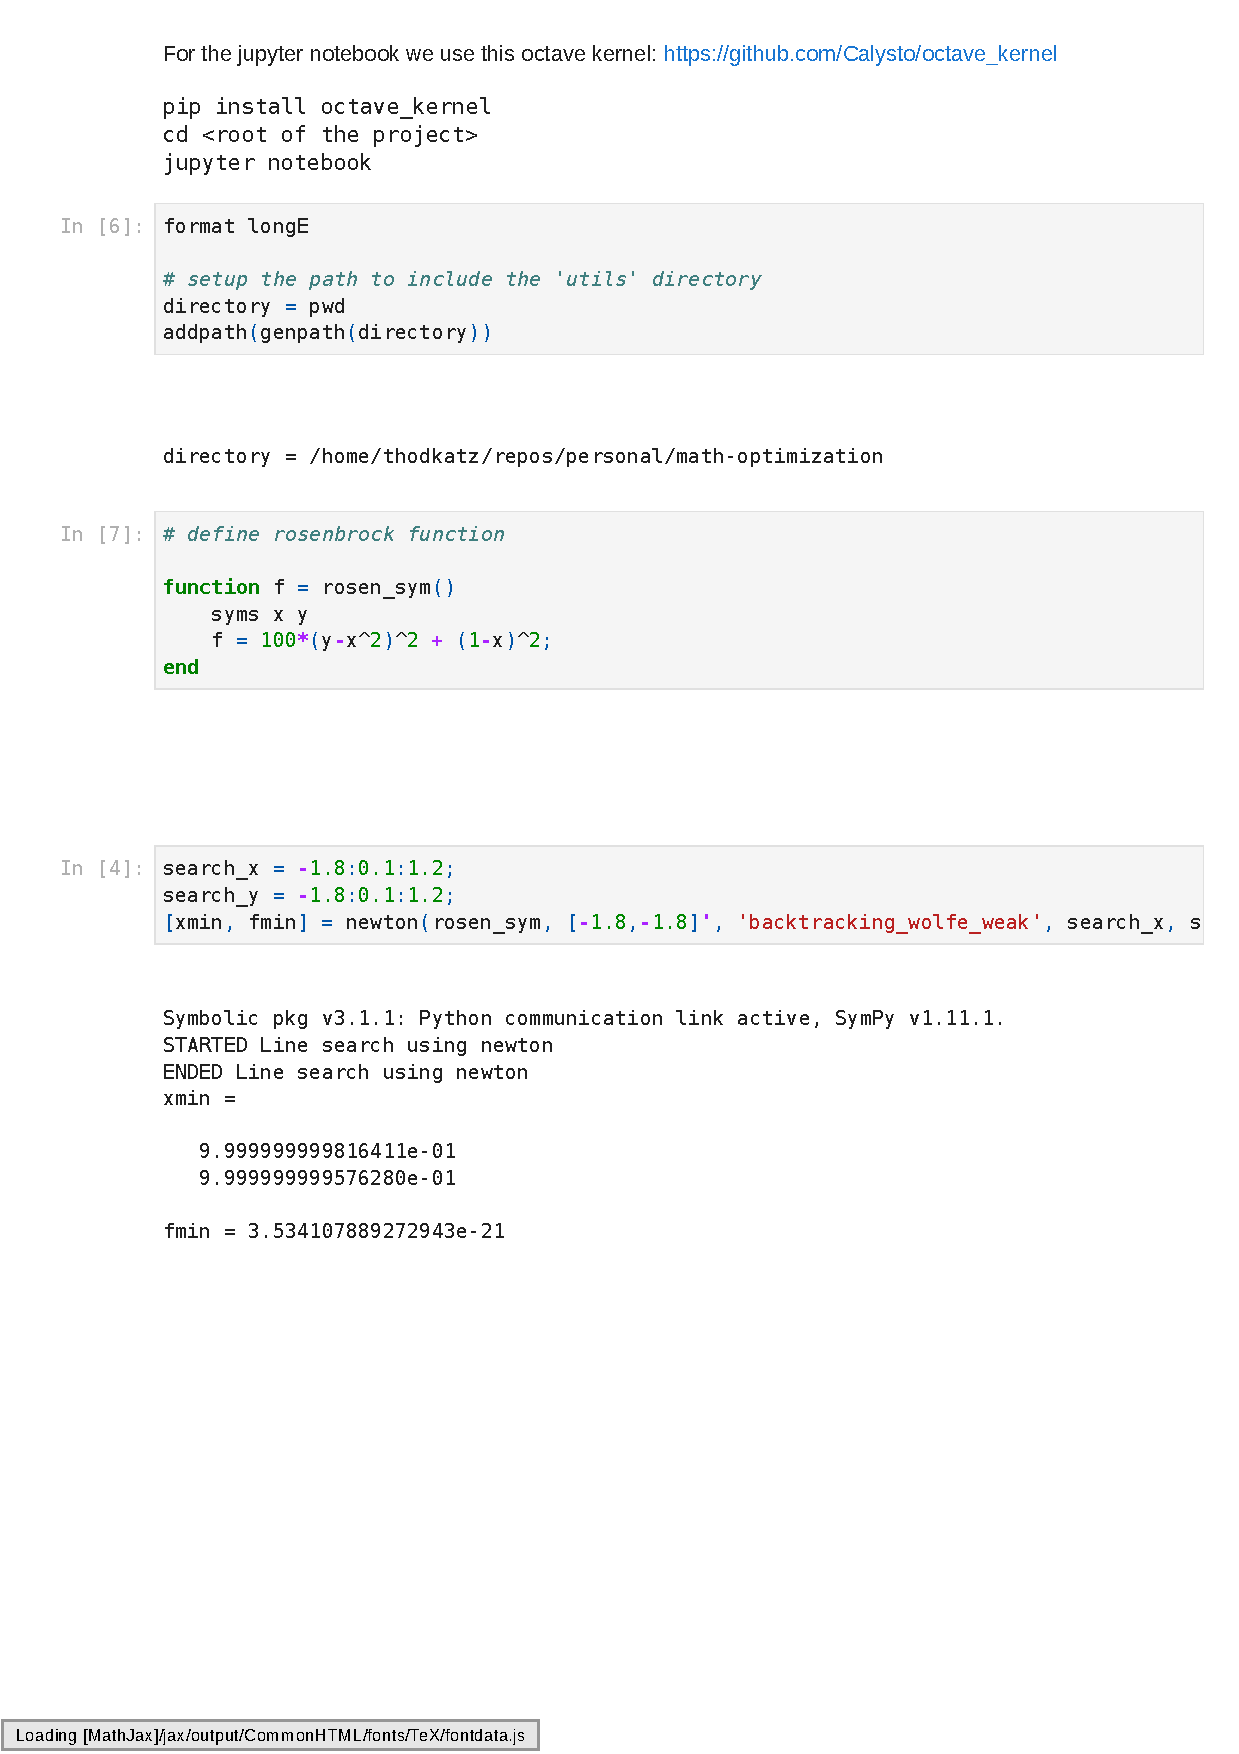
\includepdf[pages=-]{simulation.pdf}

\clearpage



\bibliographystyle{plain}
\bibliography{refs.bib}


\end{document}
